\chapter{\IfLanguageName{dutch}{Resultaten}{Results}}%
\label{ch:resultaten}

In dit hoofdstuk overloopt het onderzoek de resultaten van alle onderzoeksmethoden. Deze omvatten de requirementsanalyse, de vergelijking van taalmodellen en de ontwikkeling van \textit{Pentimentor}. Allereerst bespreekt dit hoofdstuk de resultaten van de requirementsanalyse door het moscow-schema op de uitgeteste tools toe te passen. Daarna staat het onderzoek stil bij de verkregen machinale en menselijke resultaten bij de vergelijking van vier taalmodellen. Met deze resultaten kan het onderzoek een geschikt taalmodel voor personaliseerbare \textit{automatic text simplification} (ATS) uitkiezen. Tot slot bespreekt het onderzoek het Pentimentor en vergelijkt het dit met vergelijkbare tools op basis van functionaliteiten en verschillende uitvoer. 

\medspace

Verder bevatten de resultaten enkel de belangrijkste grafieken. Alle resultaten slaat het onderzoek op in csv-bestanden. Deze bestanden kan de lezer terugvinden op de bijhorende GitHub-repository\footnote{https://github.com/dylancluyse/bachelorproef-nlp-tekstvereenvoudiging/blob/main/STATISTIEKEN\_BACHELORPROEF\_ATS.csv}.

\section{Ontbrekende functies bij AI-toepassingen}

Tabel \ref{table:afgetoetste-criteria} toont de resultaten van de requirementsanalyse.

\begin{table}[H]
	\centering
	\begin{tabular}{ | m{8cm} | m{0.5cm} | m{0.5cm} | m{0.5cm} | m{0.5cm} | m{0.5cm} | m{0.5cm} | m{1cm} | m{1cm} | }
		\hline
		\textbf{Richtlijn} & \textbf{E1} & \textbf{E2} & \textbf{E3} & \textbf{O1} & \textbf{O2} & \textbf{O3} & \textbf{O4} & \textbf{O5} \\ \hline
		Rekening houden met doelgroep & - & - & - & - & - & - & P2 & P2 \\ \hline
		Woorden met minder lettergrepen gebruiken & - & X & - & X & - & - & P1-6 & P1-6 \\ \hline
		Extra uitleg schrijven bij zinnen & - & X & - & - & - & - & P1-3 & P1-3 \\ \hline
		Paragrafen herschrijven zodat ze eerst uitleg geven op een high-level niveau & - & - & - & - & - & - & P2 & P2 \\ \hline
		Woordenlijst aanmaken & X & X & X & X & - & - & P6 & P6 \\ \hline
		Synoniemenlijst aanmaken & - & X & - & - & - & - & P6 & P6 \\ \hline
		Idiomen vervangen door eenvoudigere synoniemen & - & - & - & X & - & - & P1-3,6 & P1-3,6 \\ \hline
		Zinnen inkorten & - & - & - & X & X & X & P3-5 & P3-5 \\ \hline
		Verwijswoorden aanpassen & - & - & - & X & - & X & P3 & P3 \\ \hline
		Voorzetseluitdrukkingen aanpassen & - & - & - & - & - & - & P3 & P3 \\ \hline
		Samengestelde werkwoorden aanpassen & - & - & - & X & - & X & P3 & P3 \\ \hline
		Actieve stem toepassen & - & - & - & - & - & - & - & - \\ \hline
		Enkel regelmatige werkwoorden gebruiken & - & - & - & - & - & - & P3 & P3 \\ \hline
		Achtergrondkleur aanpassen & X & X & X & - & - & - & - & - \\ \hline
		Woord- en karakterspatiëring aanpassen & - & X & X & - & - & - & - & - \\ \hline
		Consistente lay-out & X & X & X & - & - & - & P1-6 & P1-6 \\ \hline
		Duidelijk zichtbare koppenstructuur & X & X & X & - & - & - & X & X \\ \hline
		Huidige positie benadrukken & X & X & X & - & - & - & - & - \\ \hline
		Waarschuwingen geven omtrent formulieren en sessies & - & - & - & X & - & X & - & - \\ \hline
		Inhoud visueel groeperen & - & X & X & - & - & - & - & - \\ \hline
		Tekst herschrijven als tabel & - & - & - & - & - & - & P4, P6 & P4, P6 \\ \hline
		Tekst herschrijven als opsomming & - & - & - & - & - & - & P5 & P5 \\ \hline
		Artikel opladen als pdf & X & X & X & - & X & X & - & - \\ \hline
		Artikel opladen als \textit{plain-text} & - & - & - & X & - & X & P1-6 & P1-6 \\ \hline
		Artikel opladen via link & - & - & - & - & X* & - & P1-6* & - \\ \hline
	\end{tabular}
	\caption{Afgetoetste criteria volgens de experimenten.}
	\label{table:afgetoetste-criteria}
\end{table}

\subsubsection{Experimenten op de must-have functionaliteiten}

Allereerst wijzen de experimenten uit dat niet alle toepassingen de vermelde personaliseerbare opmaakopties aanreiken. Zo beschikken enkel E1, E2 en E3 over deze opties. Andere tools bieden enkel een statische webweergave aan. Verder bieden alle uitgeteste tools een methode aan om eenduidig pdf-bestanden op te slaan, met uitzondering op O1, O4 en O5. Deze uitvoerbestanden ontbreken echter een duidelijke titelstructuur en deze kunnen eindgebruikers niet eenduidig als word-bestand raadplegen. Verder kunnen gebruikers met de geteste toepassingen een wetenschappelijk artikel als pdf opladen. Uitzonderlijk laten O4 en O5 dit niet toe. Zij werken enkel met tekstinvoer. Figuur \ref{img:scispace-example} toont de werking van toepassing O2. Deze figuur toont hoe een eindgebruiker de tekst van het oorspronkelijk pdf-bestand kan selecteren. Vervolgens kunnen zij dit eenvoudig laten samenvatten door de toepassing. Tot slot kunnen zij uitzonderlijk met O2 en O5 online wetenschappelijke artikelen via URL opladen.

\begin{figure}[H]
	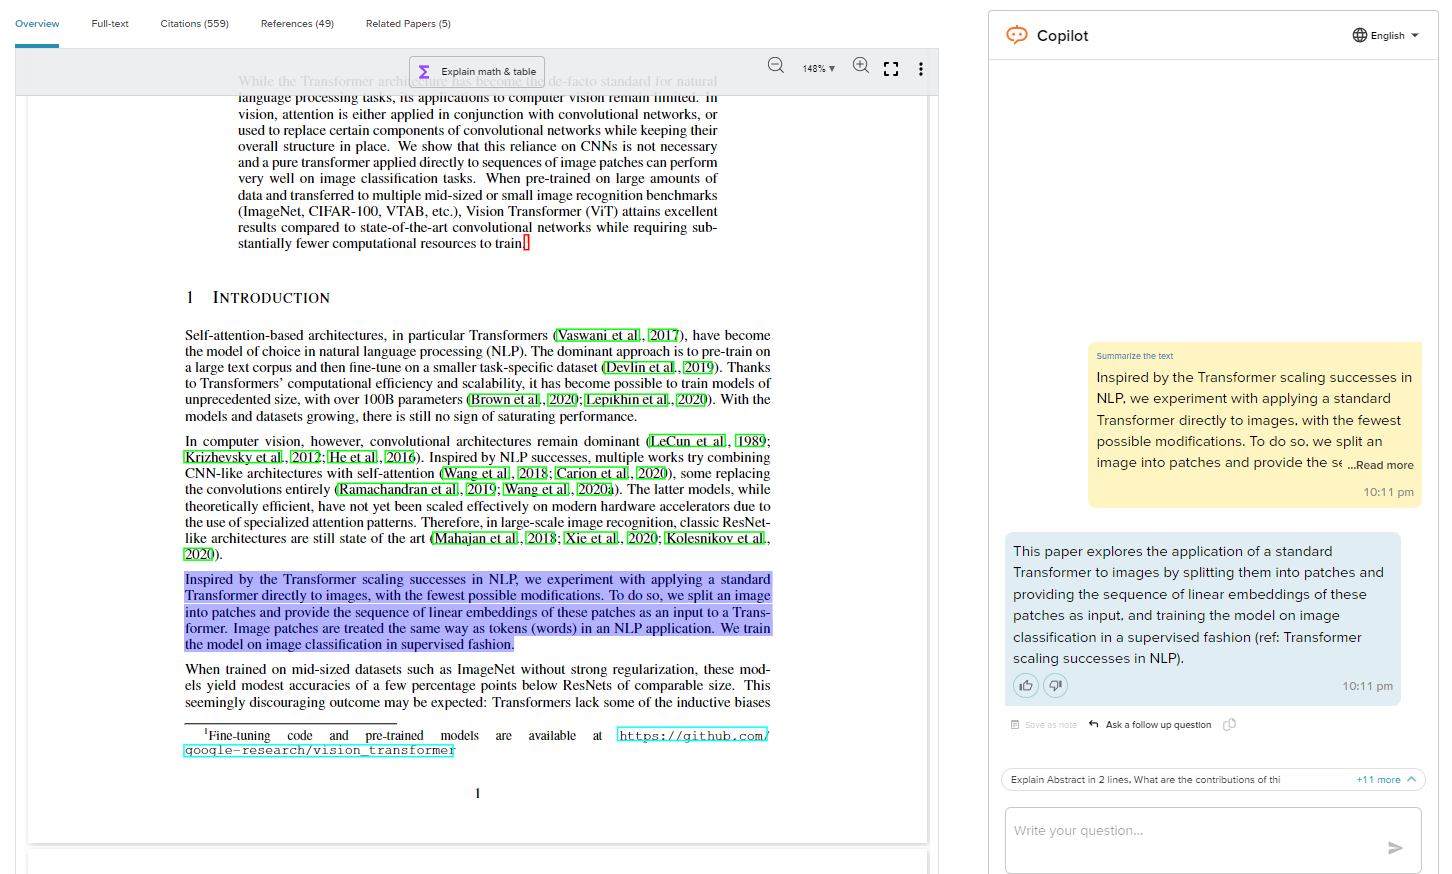
\includegraphics[width=\linewidth]{img/typeset-example.png}
	\caption{Informatie opvragen van een wetenschappelijk artikel met SciSpace}
	\label{img:scispace-example}
\end{figure}

Verder moeten toepassingen een moeilijk woord in een doorlopende tekst kunnen aanpassen. Specifiek kunnen O1, O3, O4 en O5 een annotatie toevoegen aan moeilijke woorden, maar dit gebeurt alleen als er daarvoor geen geschikt synoniem beschikbaar is. Zo illustreert figuur \ref{img:simplish-output} hoe O1 een extra definitie als annotatie kan geven. Hoewel dit het taalniveau niet kan aanpassen, toch laat figuur \ref{img:scholarcy} zien hoe O3 dit probeert in te schatten met een \textit{rewordifying level}. Bovendien kunnen O4 en O5 de doelgroep aanpassen afhankelijk van de \textit{prompts}. Andere uitgeteste tools tonen niet hoe zij de doelgroepinschatting maken. Geen tool laat gebruikers toe om een vooraf opgestelde woordenlijst met moeilijke woorden mee te geven waarop de tool zich kan baseren.

\begin{figure}[H]
	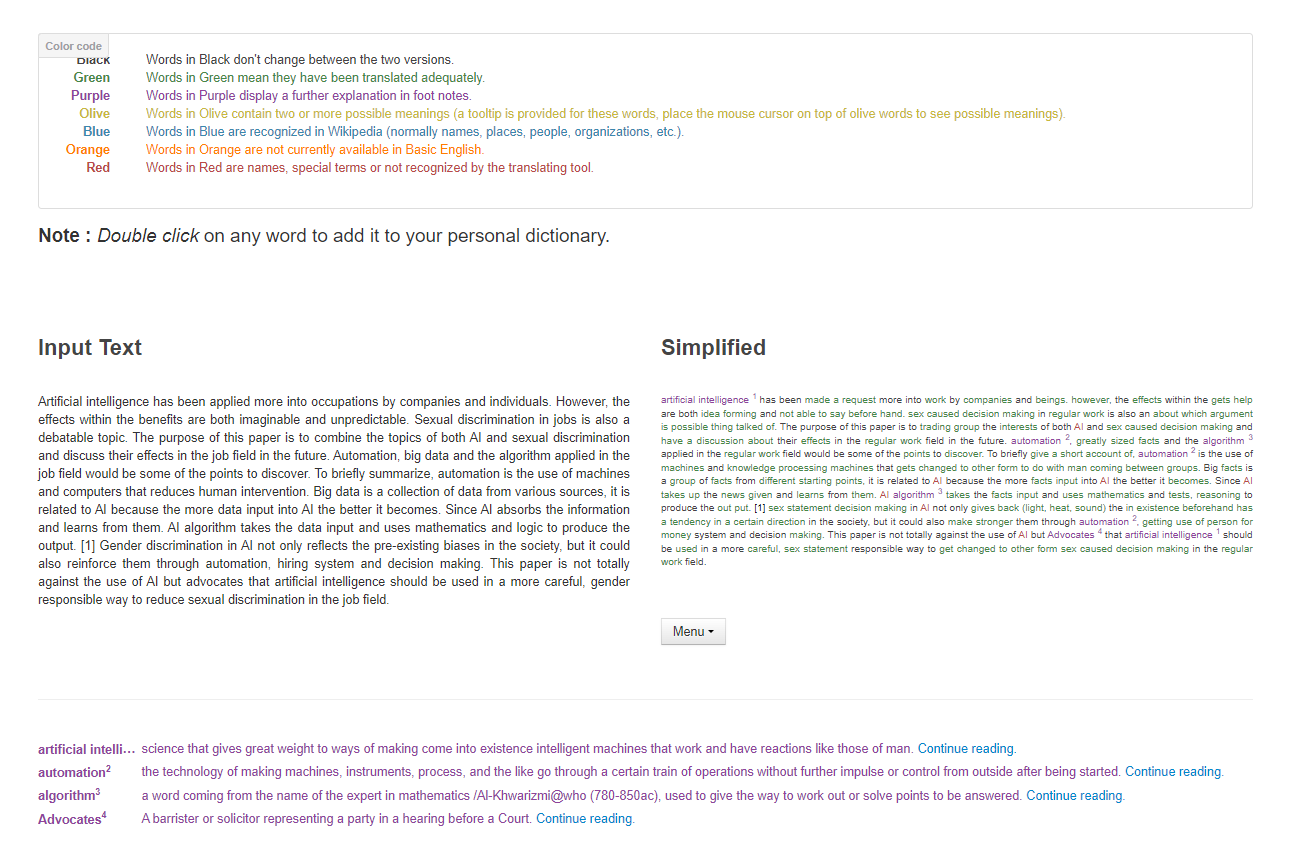
\includegraphics[width=\linewidth]{img/simplish-output.png}
	\caption{Schermafbeelding van de tekstanalyse bij Simplish na een tekstvereenvoudiging.}
	\label{img:simplish-output}
\end{figure}

Daarnaast kunnen toepassingen ook handmatig een woordenlijst maken. Zo kunnen E1, E2, E3 en O1 een woorden- of synoniemenlijst opstellen. Bij deze toepassingen selecteren gebruikers handmatig moeilijke woorden. Die moet de toepassing vereenvoudigen of een definitie ervan ophalen. Uitzonderlijk O1 geeft de woordsoort mee. Verder kunnen gebruikers niet bepalen uit welke bron de definitie moet komen, bijvoorbeeld een online woordenboek. Enkel E1 laat dit toe.

\medspace

Verder kunnen E1, E2 en E3 geen syntactische vereenvoudiging toepassen op de oorspronkelijke tekst. Overige uitgeteste tools kunnen zinnen inkorten door deze te splitsen. Geen van de uitgeteste tools kunnen de geselecteerde tekst automatisch naar een actieve vorm schrijven. In tegenstelling tot O4 en O5 die dit wel kunnen doen, maar enkel als de tool een onderwerp in de prompt meekrijgt. 

\medspace

Tot slot slagen O2, O4 en O5 erin om de tekst te herschrijven als opsomming. Zo doet O2 dit automatisch, vergeleken met O4 en O5 die deze vraag expliciet in hun prompt moeten krijgen. De andere uitgeteste tools kunnen dit niet automatisch doen. 

\subsubsection{Should-haves}

Allereerst tonen O1 en O3 automatisch leesgraadmetrieken nadat die een vereenvoudiging of samenvatting maken van de oorspronkelijke tekst. Zo tonen figuren \ref{img:simplish-output} en \ref{img:scholarcy} een voorbeeld van deze analyse. Deze analyse toont het aantal zinnen en complexe/lange woorden voor zowel het oorspronkelijk als het vereenvoudigde artikel. Andere uitgeteste tools tonen dit niet.

\begin{figure}[H]
	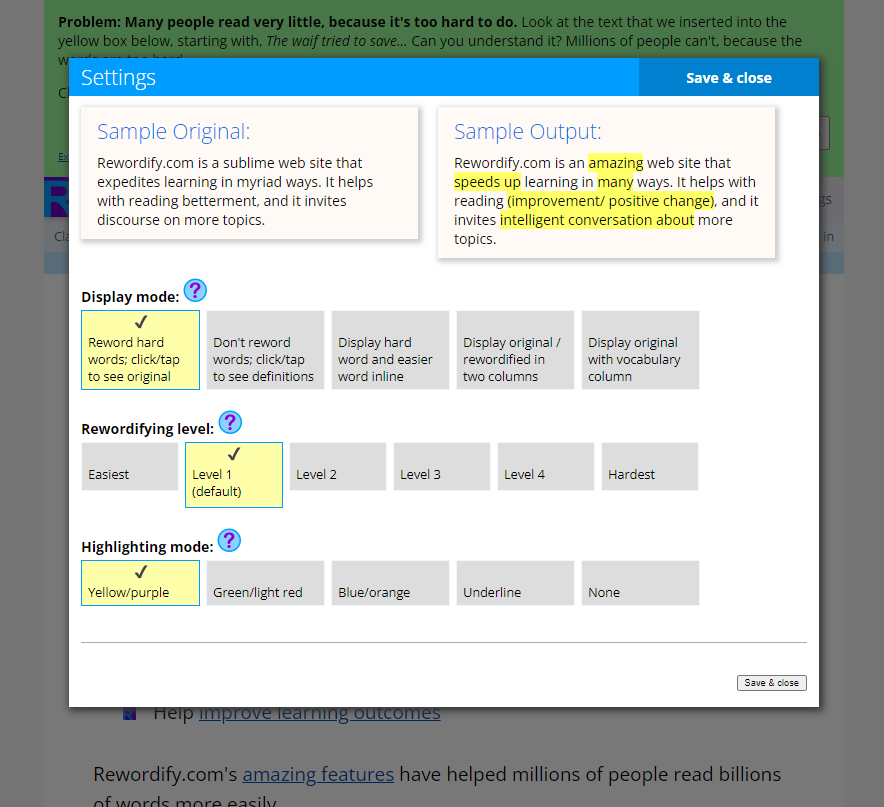
\includegraphics[width=\linewidth]{img/scholarcy-attempt.png}
	\caption{Tekstanalyse met \textit{Rewordify}.}
	\label{img:scholarcy}
\end{figure}

Verder kan het onderzoek niet afleiden of de uitgeteste tools een OCR-techniek gebruiken. Wel gebruikt O2 een andere inleestechniek dan de andere tools. Zo kan het de twee gebruikte wetenschappelijke artikelen inlezen met een identieke lay-out als het oorspronkelijk artikel. Daarna markeert de gebruiker enkel aanpassingen in het artikel, terwijl alle uitvoer van het taalmodel rechts in beeld komt. Echter, de gebruiker kan deze aanpassing niet afleiden uit de oorspronkelijke tekst, in tegenstelling tot O1 en O3. Die tonen wel de verschillen tussen het oorspronkelijk en het vereenvoudigd artikel aan de eindgebruiker.

\subsubsection{Could-haves}

Verschillende geteste tools maken gebruik van gebruikerfeedbacktechnieken in de vorm van \textit{pop-ups}, zoals bij een aanpassing van de tekst. O4 en O5 vormen hierop een uitzondering, omdat zij deze technieken niet bevatten. Uitzonderlijk O4 en O5 kunnen tekst omzetten naar een tabelformaat, maar dit gebeurt alleen na een expliciete prompt. Ze hebben de mogelijkheid om tekst te interpreteren en deze in een tabel te gieten. Zo maken ze gebruik van een 2 op 2 tabel, maar de gebruiker kan het aantal kolommen en rijen instellen via de prompt.

\medspace

Geen van de geteste tools kan automatisch moeilijke woorden of vakterminologie extraheren uit een tekst, behalve O4 en O5, die dit wel kunnen met behulp van een expliciete prompt.

\medspace

Wat betreft samenvattingen kunnen O1, O2, O3, O4 en O5 zowel extraherende als abstraherende samenvattingen maken van de oorspronkelijke tekst. E1, E2 en E3 kunnen alleen een extraherende samenvatting maken, maar dit gebeurt pas na een handmatige selectie van de zinnen.

\medspace

Alleen O4 en O5 hebben de mogelijkheid om een gegeven tekst te herschrijven. Dezelfde prompt kan leiden tot een ontelbaar aantal resultaten. Alle andere toepassingen slagen hier niet in en alle versies van een herschreven artikel leiden tot hetzelfde resultaat. Tot slot kunnen enkel O1, O2, O4 en O5 wel onregelmatige werkwoorden corrigeren.

\subsubsection{Wont-haves}

Op het vlak van toegankelijkheid beschikken O4 en O5 over een mobiele versie. Daarnaast kan een gebruiker O1, O2 en O3 wel via een mobiel apparaat bekijken, maar deze lenen geen speciale interface toe. Vervolgens bieden E1, E2 en E3 geen mobiele versie aan. 

\medspace

Daarnaast beschikken enkel E1, E2 en E3 over luistersoftware. Hoewel browsers over ingebouwde luistertools beschikken, toch bieden de andere tools geen personaliseerbare \textit{text-to-speech} techniek aan. Tot slot beschikken de geteste toepassingen over geen integratie met andere spelcheckers. Wel werkt de browserextensie van \textit{Grammarly} bij zowel O1, O2, O3, O4 en O5. 

\section{Geschikte taalmodel voor gepersonaliseerde tekstvereenvoudiging met ATS}

De vergelijkende studie evalueert de uitvoer van de uitgeteste taallmodellen, opgesomd in \ref{table:vergelijkende-studie-taalmodellen}, met een machinale en een menselijke beoordeling. Zo achterhaalt deze onderzoeksmethode welk taalmodel of LLM beter aansluit bij het aanbieden van gepersonaliseerde ATS voor scholieren met dyslexie in de derde graad van het middelbaar onderwijs. 

\subsubsection{Machinale beoordeling van de vereenvoudigde teksten}

Tabel \ref{table:resultaten-aantal-zinnen} geeft het aantal zinnen per (vereenvoudigd) artikel. De MTS-referentieteksten bevatten minder zinnen dan het oorspronkelijk artikel. Het aantal zinnen na ATS met T1, T2 en T3 is gehalveerd tot minder dan een kwart van oorspronkelijke hoeveelheid zinnen. Enkel T4P2 genereert meer zinnen dan de oorspronkelijke versie van A1 na ATS. T4P2 genereert bij zowel A1 als A2 meer zinnen vergeleken met de andere geteste taalmodellen. T2 daarentegen genereert bij beide artikelen het minst aantal zinnen. Figuren \ref{img:boxplot-min-max-avg-words-a1} en \ref{img:boxplot-min-max-avg-words-a2} illustreren deze verschillen tussen de taalmodellen.

\begin{table}[h]
	\centering
	\begin{tabular}{ | m{3cm} | m{3cm} | m{3cm} | } 
		\hline
		\textbf{Bron} & \textbf{#Zinnen in A1} & \textbf{#Zinnen in A2} \\
		\hline
		Oorspronkelijk & 78  & 159 \\ 
		\hline
		MTS (door leerkracht) & 43 & 45 \\
		\hline
		MTS (door leerling) & n.v.t. & 50 \\
		\hline
		T1 & 26 & 24 \\
		\hline
		T2 & 11 & 7 \\
		\hline
		T3 & 67 & 130 \\
		\hline
		T4 P1 & 61 & 98 \\
		\hline
		T4 P2 & 89 & 133 \\
		\hline
		T4 P3 & 39 & 55 \\
		\hline
	\end{tabular}
	\caption{Aantal zinnen (gemeten met Spacy sentence embeddings) per tekst.}
	\label{table:resultaten-aantal-zinnen}
\end{table}

\begin{figure}[H]
	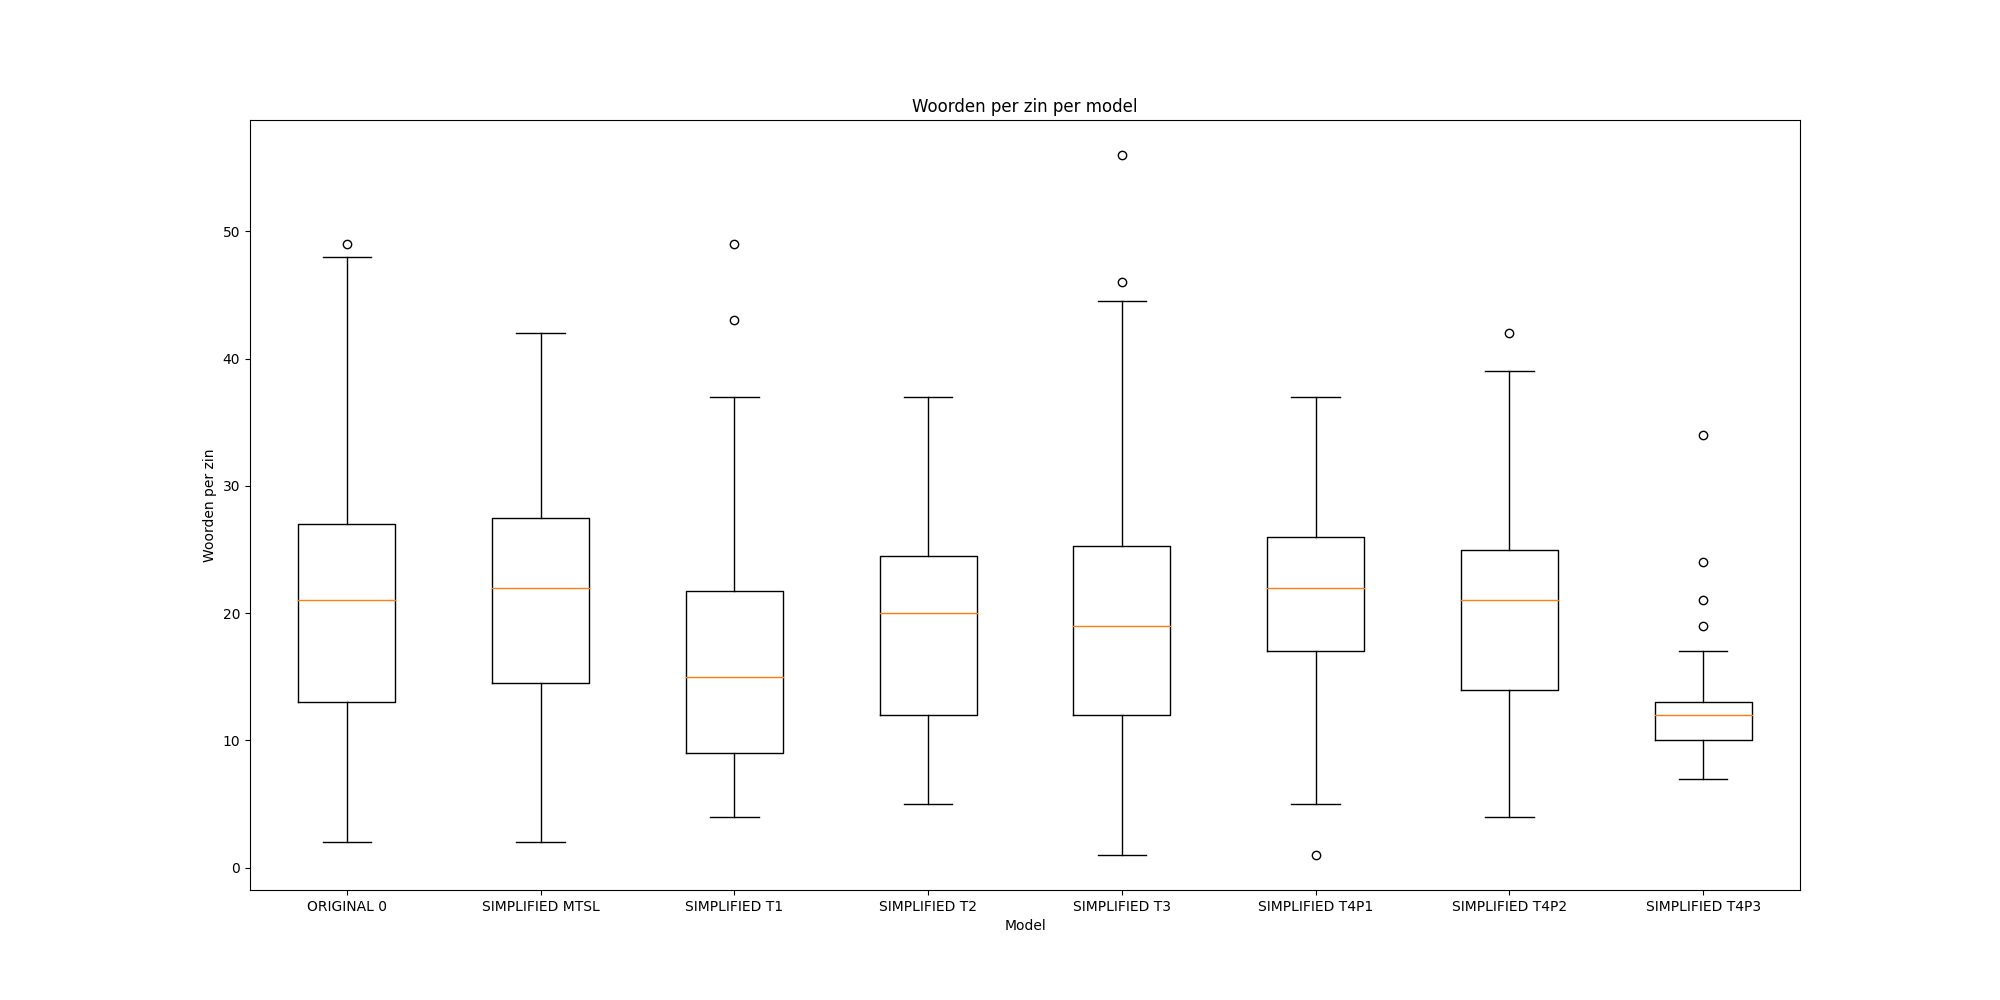
\includegraphics[width=\linewidth]{img/boxplot-avg-a1.png}
	\caption{Overzicht van het minimum, maximum en gemiddeld aantal woorden per zin per model in A1.}
	\label{img:boxplot-min-max-avg-words-a1}
\end{figure}

\begin{figure}[H]
	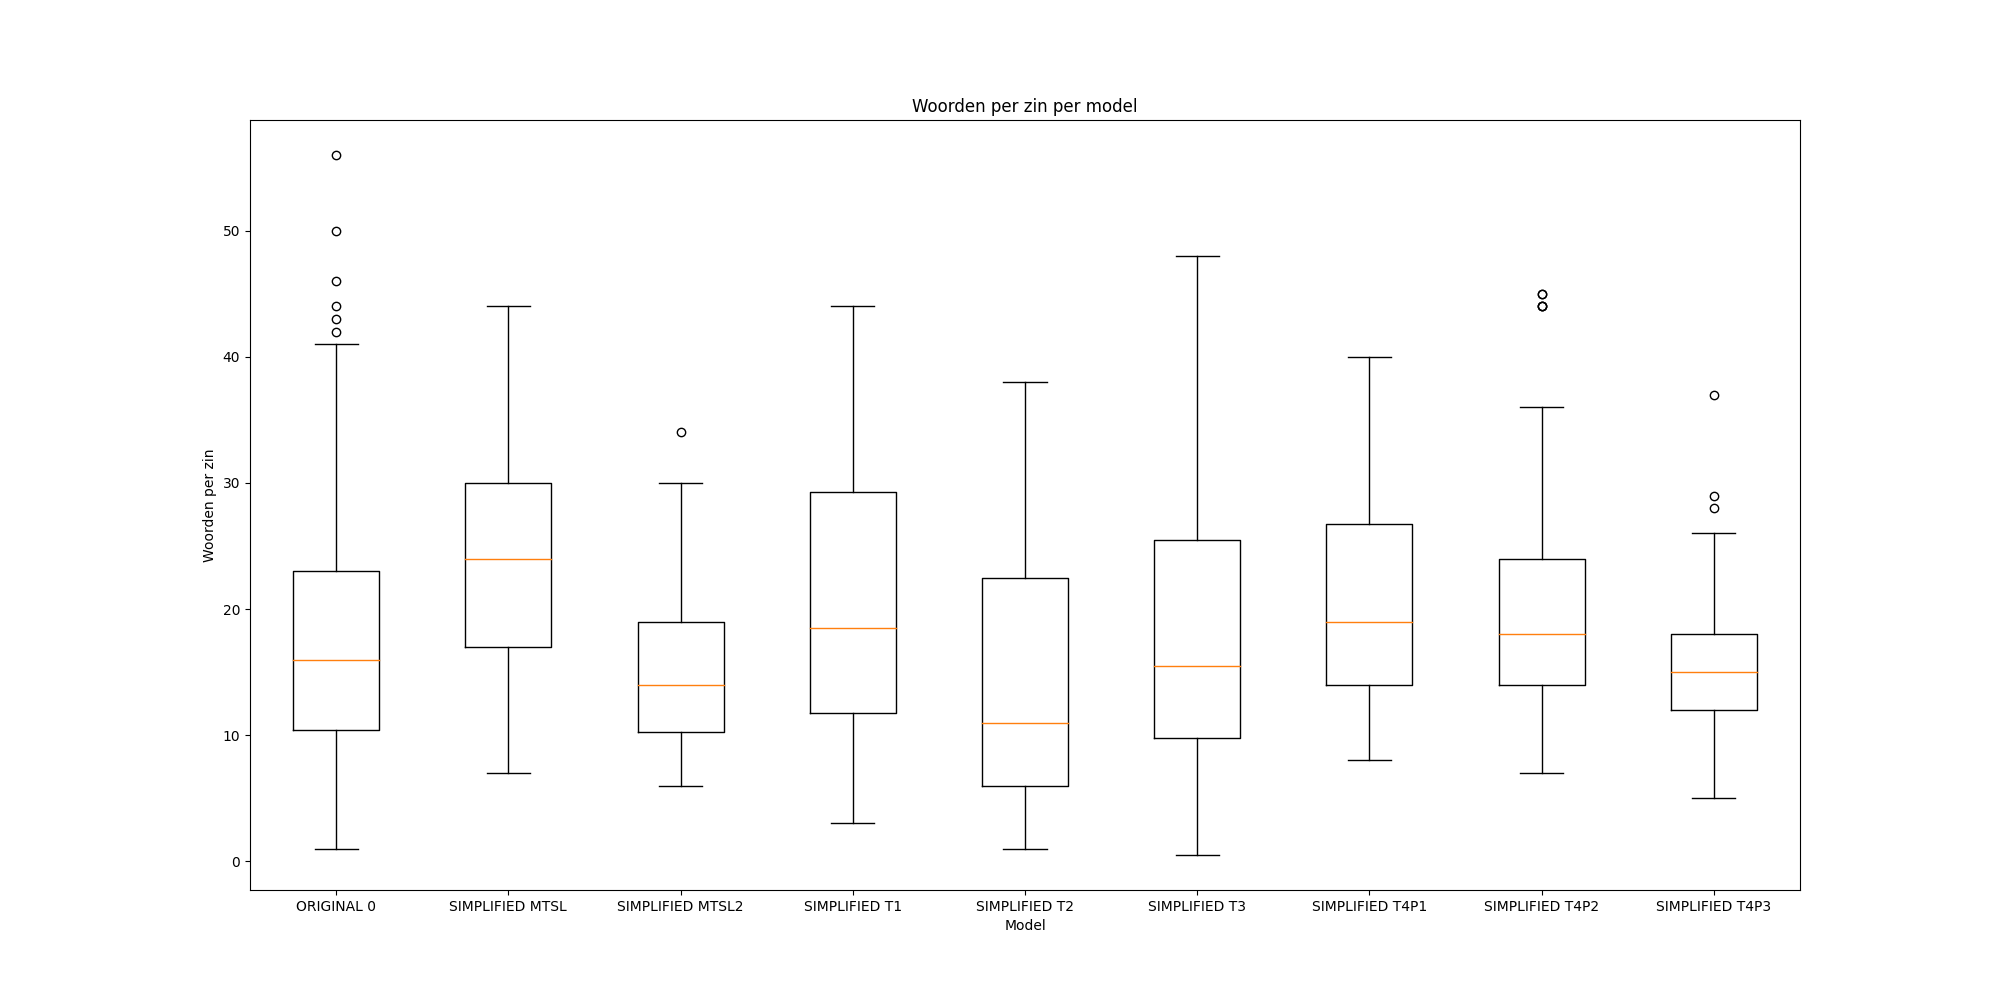
\includegraphics[width=\linewidth]{img/boxplot-avg-a2.png}
	\caption{Overzicht van het minimum, maximum en gemiddeld aantal woorden per zin per model in A2.}
	\label{img:boxplot-min-max-avg-words-a2}
\end{figure}

Verder vergelijkt het onderzoek de verkregen leesbaarheidsscores per zin dat ieder taalmodel kan genereren. Allereerst de FRE-scores die de leesgraad van een zin aanduidt. Alle geteste taalmodellen genereren zinnen waarvan de FRE-scores niet opmerkelijk hoger of lager zijn ten opzichte van het oorspronkelijk artikel. Figuren \ref{img:boxplot-fre-a1} en \ref{img:boxplot-fre-a2} tonen deze verschillen. Gemiddeld bevinden alle versies van het wetenschappelijk artikel zich tussen 20 en 50. Zonder \textit{outliers} beperkt T3 de FRE van alle zinnen tot hoogstens 40. T3, T4P1, T4P2 en T4P3 genereren zinnen met een hogere FRE dan OG en MTSL. 

\begin{figure}[H]
	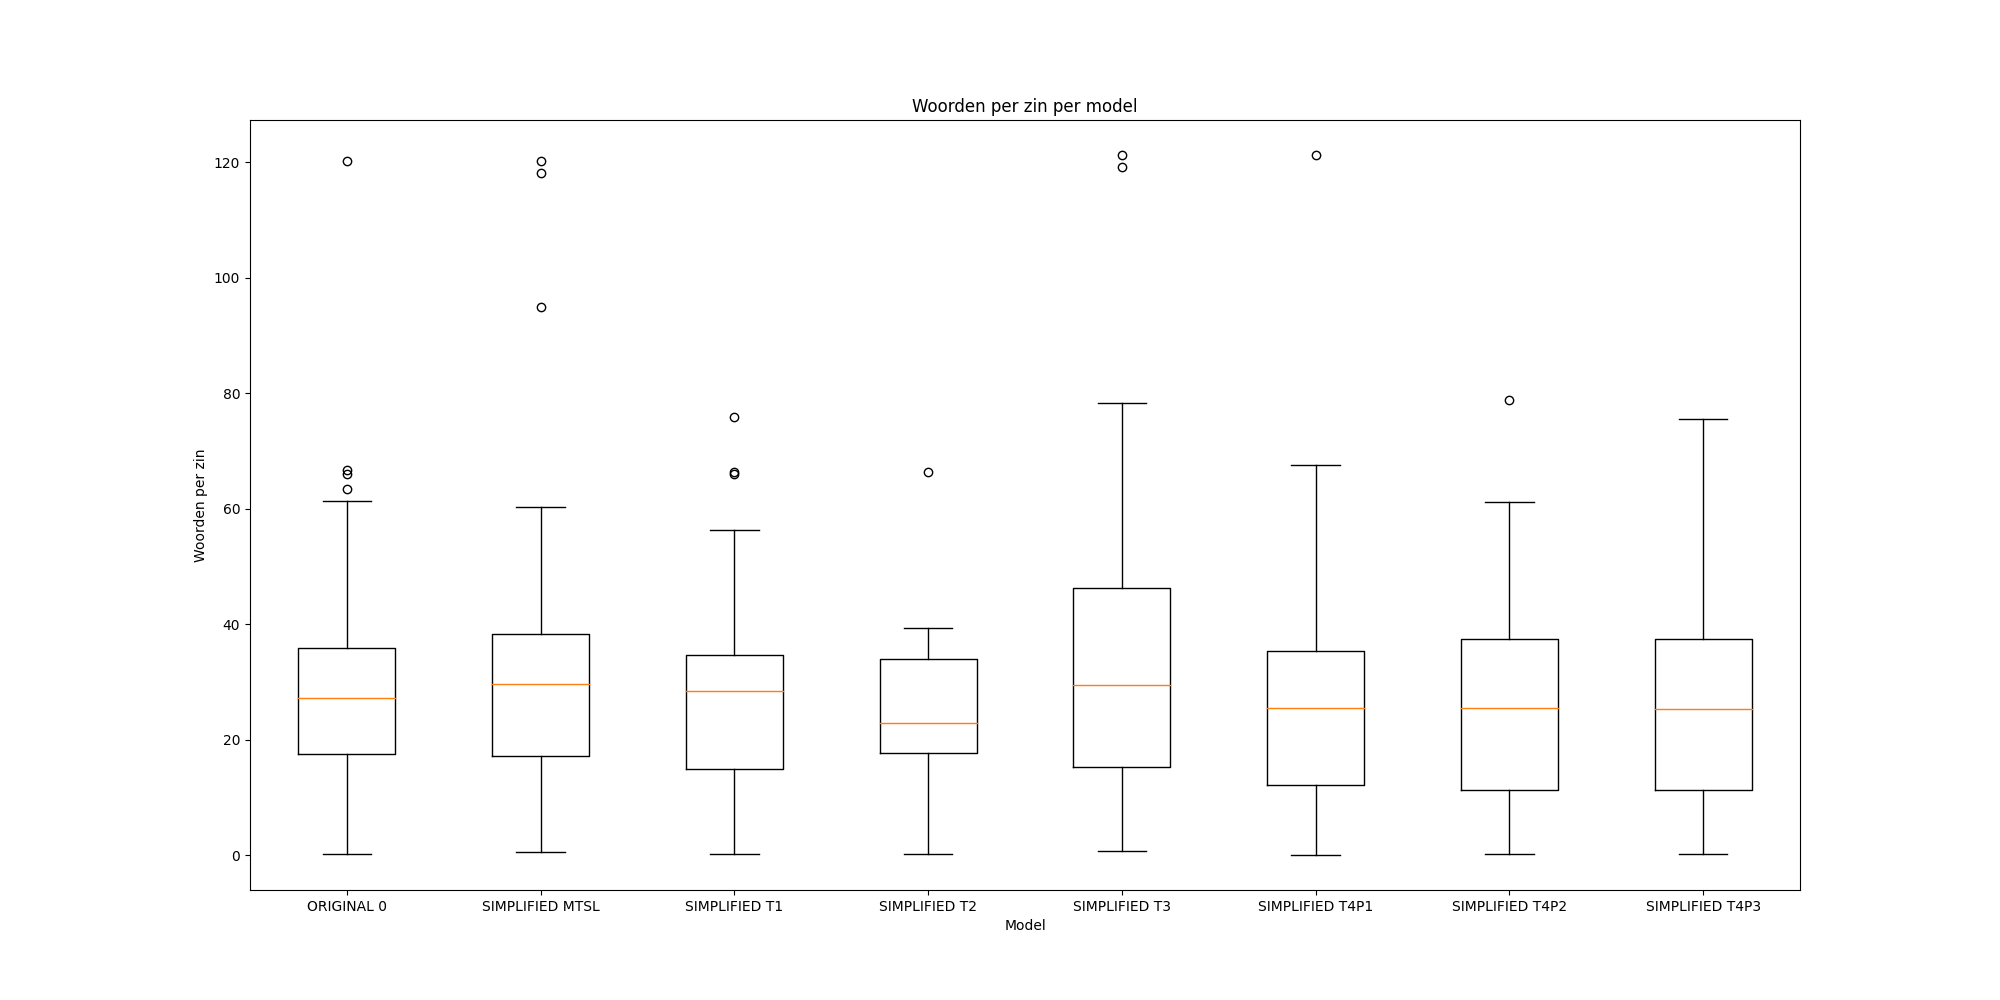
\includegraphics[width=\linewidth]{img/boxplot-fre-a1.png}
	\caption{Boxplot van de FRE-scores voor A1.}
	\label{img:boxplot-fre-a1}
\end{figure}

\begin{figure}[H]
	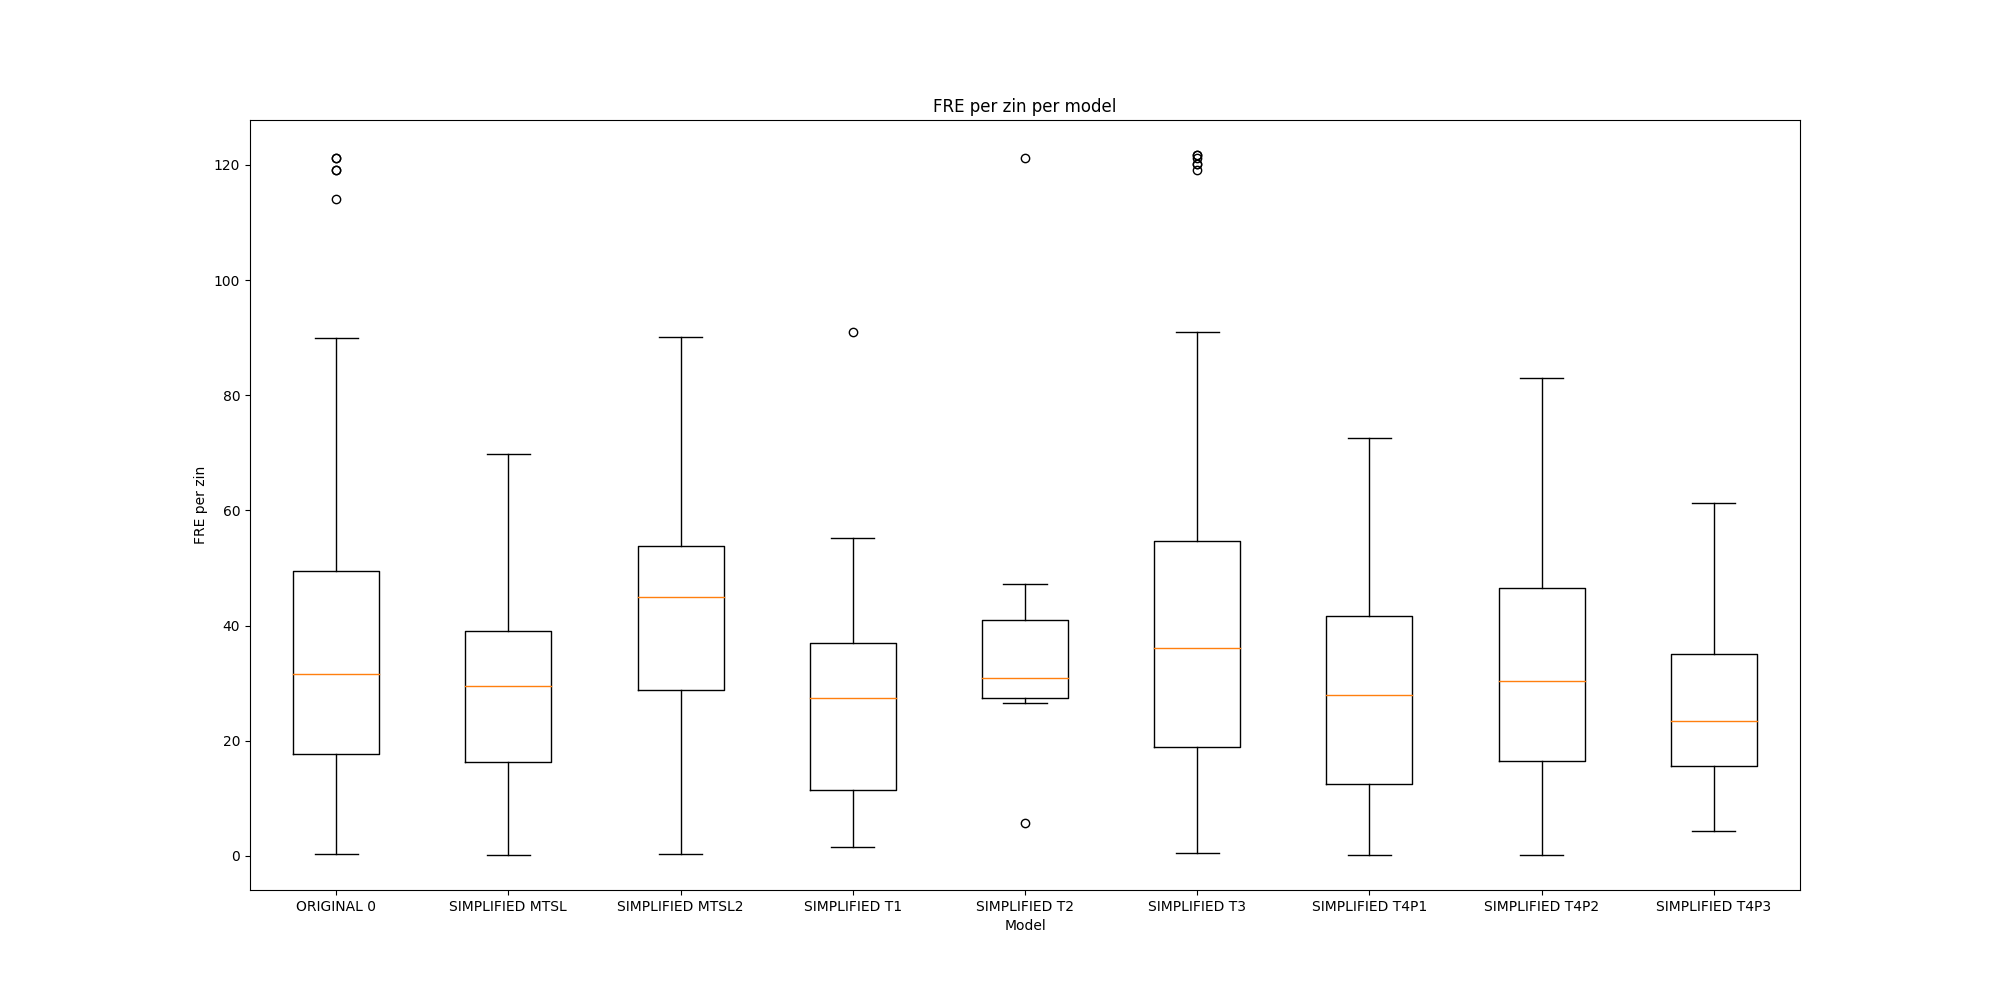
\includegraphics[width=\linewidth]{img/boxplot-fre-a2.png}
	\caption{Boxplot van de FRE-scores voor A2.}
	\label{img:boxplot-fre-a2}
\end{figure}

De FOG-scores van alle geteste taalmodellen en MTS-referentieteksten zijn niet opmerkelijk hoger of lager bij de vereenvoudigde wetenschappelijke artikelen, zoals weergegeven in figuren \ref{img:boxplot-fog-a1} en \ref{img:boxplot-fog-a2}. De zinnen van MTSL2 en T2 scoren gemiddeld lagere FOG-scores dan OG. Daarnaast scoort T2 een lager gemiddelde dan andere taalmodellen. Dit gemiddelde ligt tussen 10 en 12. Tot slot scoren MTSL en andere taalmodellen gemiddeld hoger dan OG. Tot slot genereren de taalmodellen geen zinnen met een hogere FOG-score dan OG.

\begin{figure}[H]
	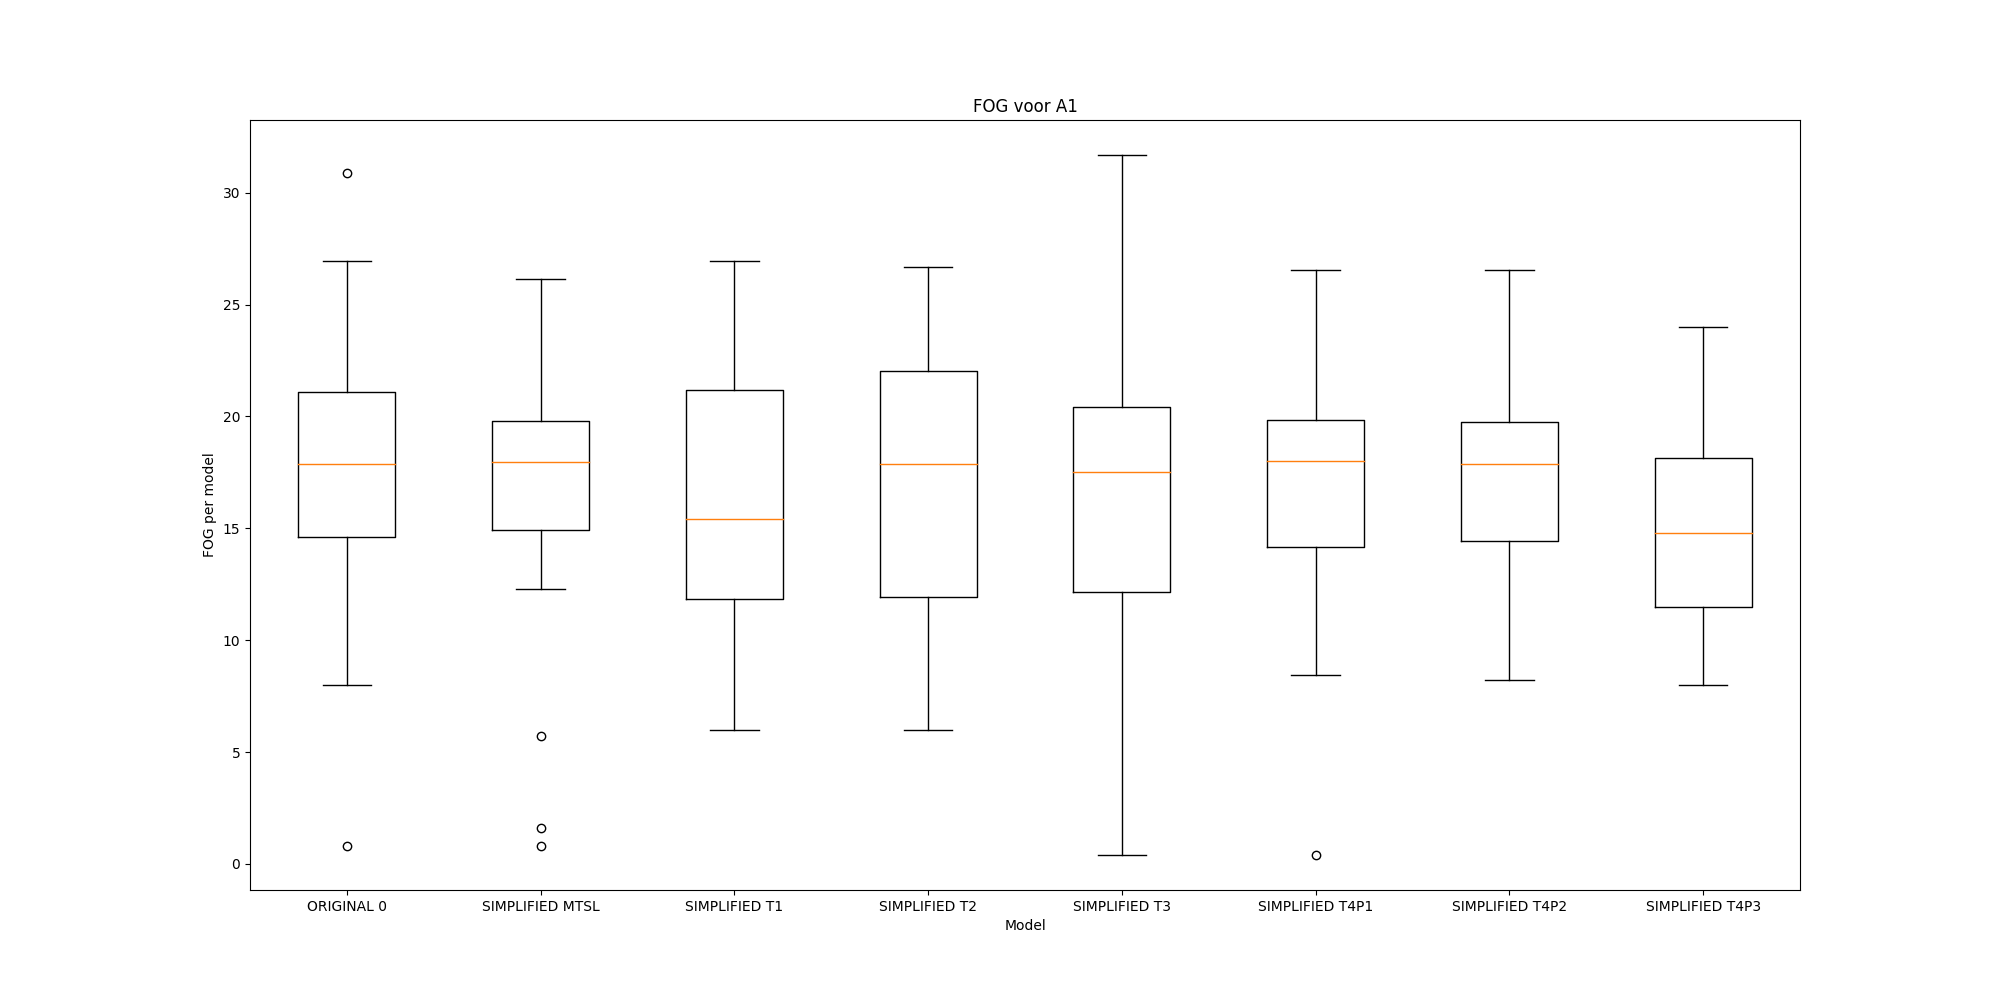
\includegraphics[width=\linewidth]{img/boxplot-fog-a1.png}
	\caption{Boxplot van de FOG-scores voor A1.}
	\label{img:boxplot-fog-a1}
\end{figure}

\begin{figure}[H]
	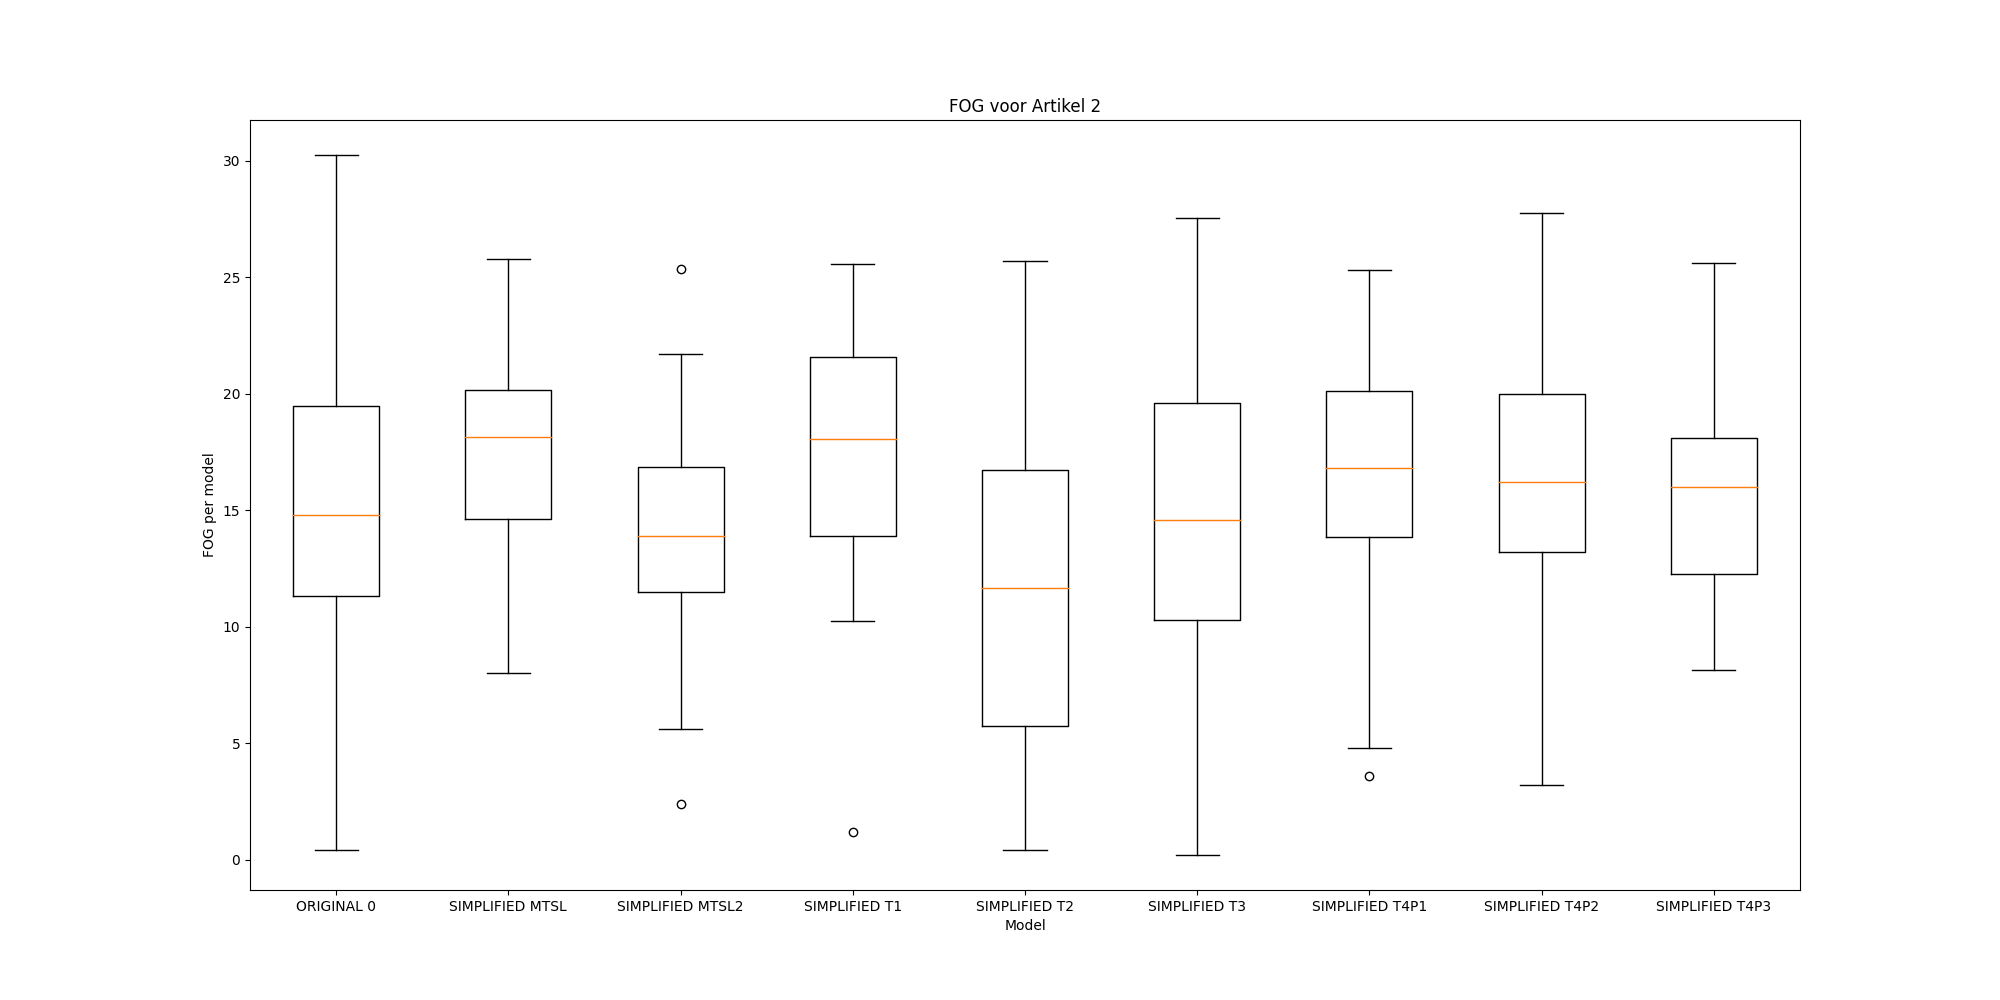
\includegraphics[width=\linewidth]{img/boxplot-fog-a2.png}
	\caption{Boxplot van de FOG-scores voor A2.}
	\label{img:boxplot-fog-a2}
\end{figure}

T1, T2 en T3 genereren meer complexe woorden vergeleken met T4, MTSL en OG. Bij A1 genereert T4P3 opmerkelijk minder complexe woorden per zin dan de andere taalmodellen. Bij A2 is er geen opmerkelijk verschil tussen de taalmodellen. Vervolgens visualiseren figuren \ref{img:violinplot-long-a1} en \ref{img:violinplot-long-a2} het aantal lange woorden per zin. Het systeem betrekt een woord met minstens vier lettergrepen als een lang woord. MTSL, T2, T4P1, T4P2 en T4P3 genereren minder lange woorden per zin dan OG.

\begin{figure}[H]
	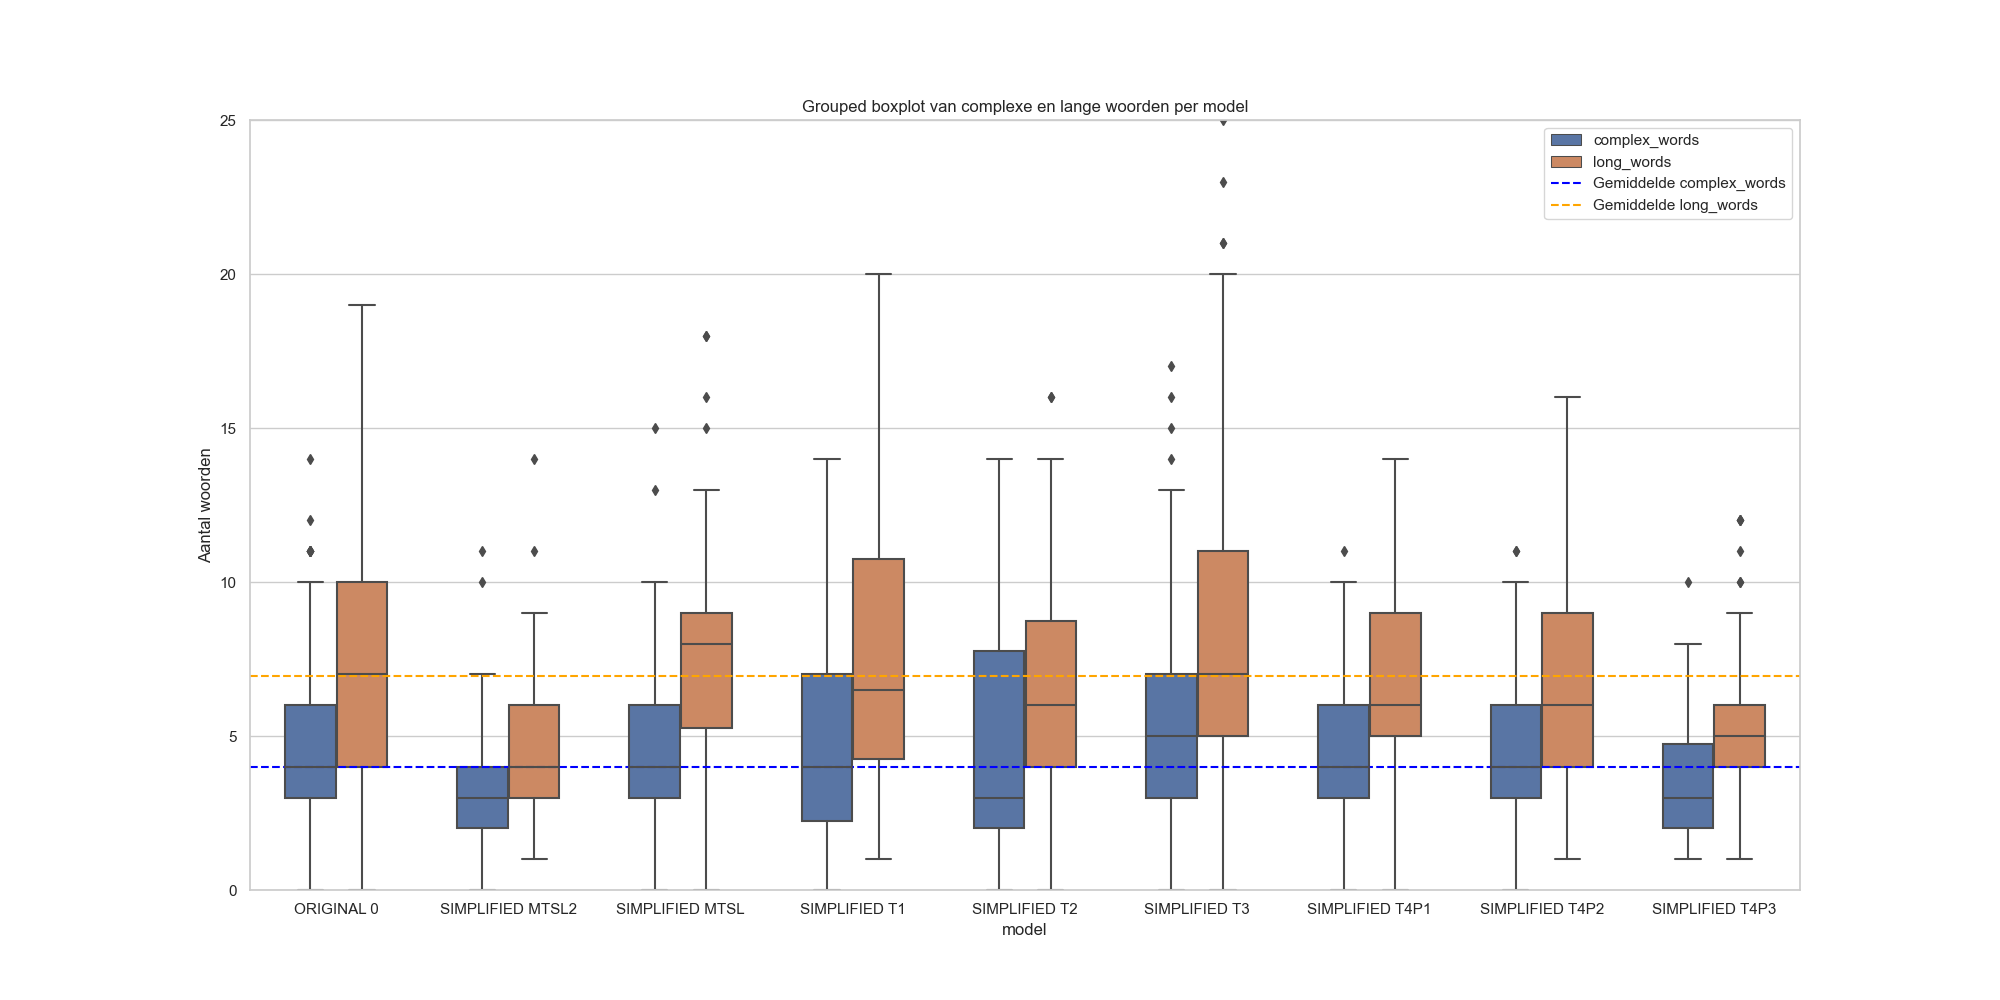
\includegraphics[width=\linewidth]{img/boxplot-poster.png}
	\caption{Een boxplot van het aantal lange en complexe woorden per zin, gegroepeerd op model voor A1.}
	\label{img:long-complex-words}
\end{figure}


Vervolgens tonen figuren \ref{img:histplot-aux-a1} en \ref{img:histplot-aux-a2} het aantal hulpwerkwoorden in de tekst. Deze figuren zijn geen absolute percentages en houden geen rekening met het aantal zinnen. Ten slotte tonen \ref{img:histplot-aux-a1} en \ref{img:histplot-aux-a2} het aantal vervoegingen van het werkwoord 'zijn' aan. 

\begin{figure}[H]
	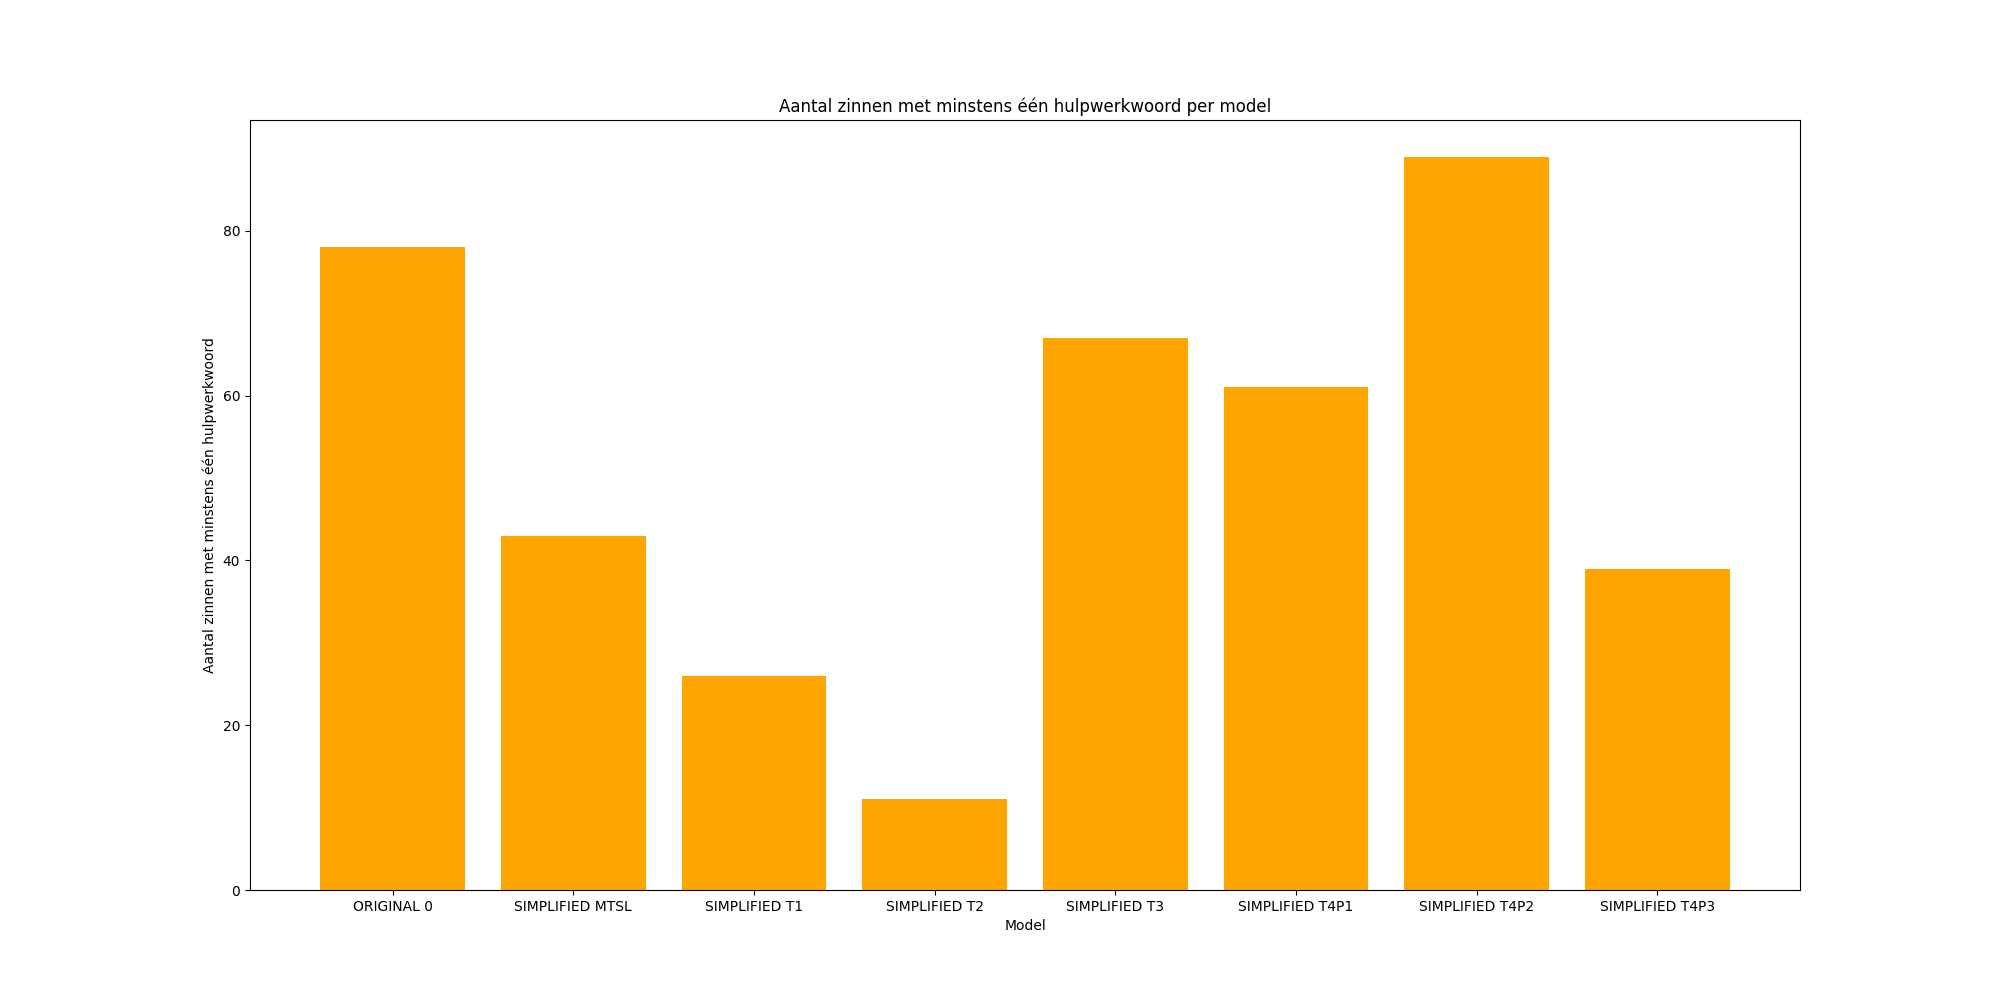
\includegraphics[width=\linewidth]{img/boxplot-aux-a1.png}
	\caption{Een staafdiagram van het aantal gebruikte hulpwerkwoorden in de tekst, gegroepeerd op model voor A1.}
	\label{img:histplot-aux-a1}
\end{figure}

\begin{figure}[H]
	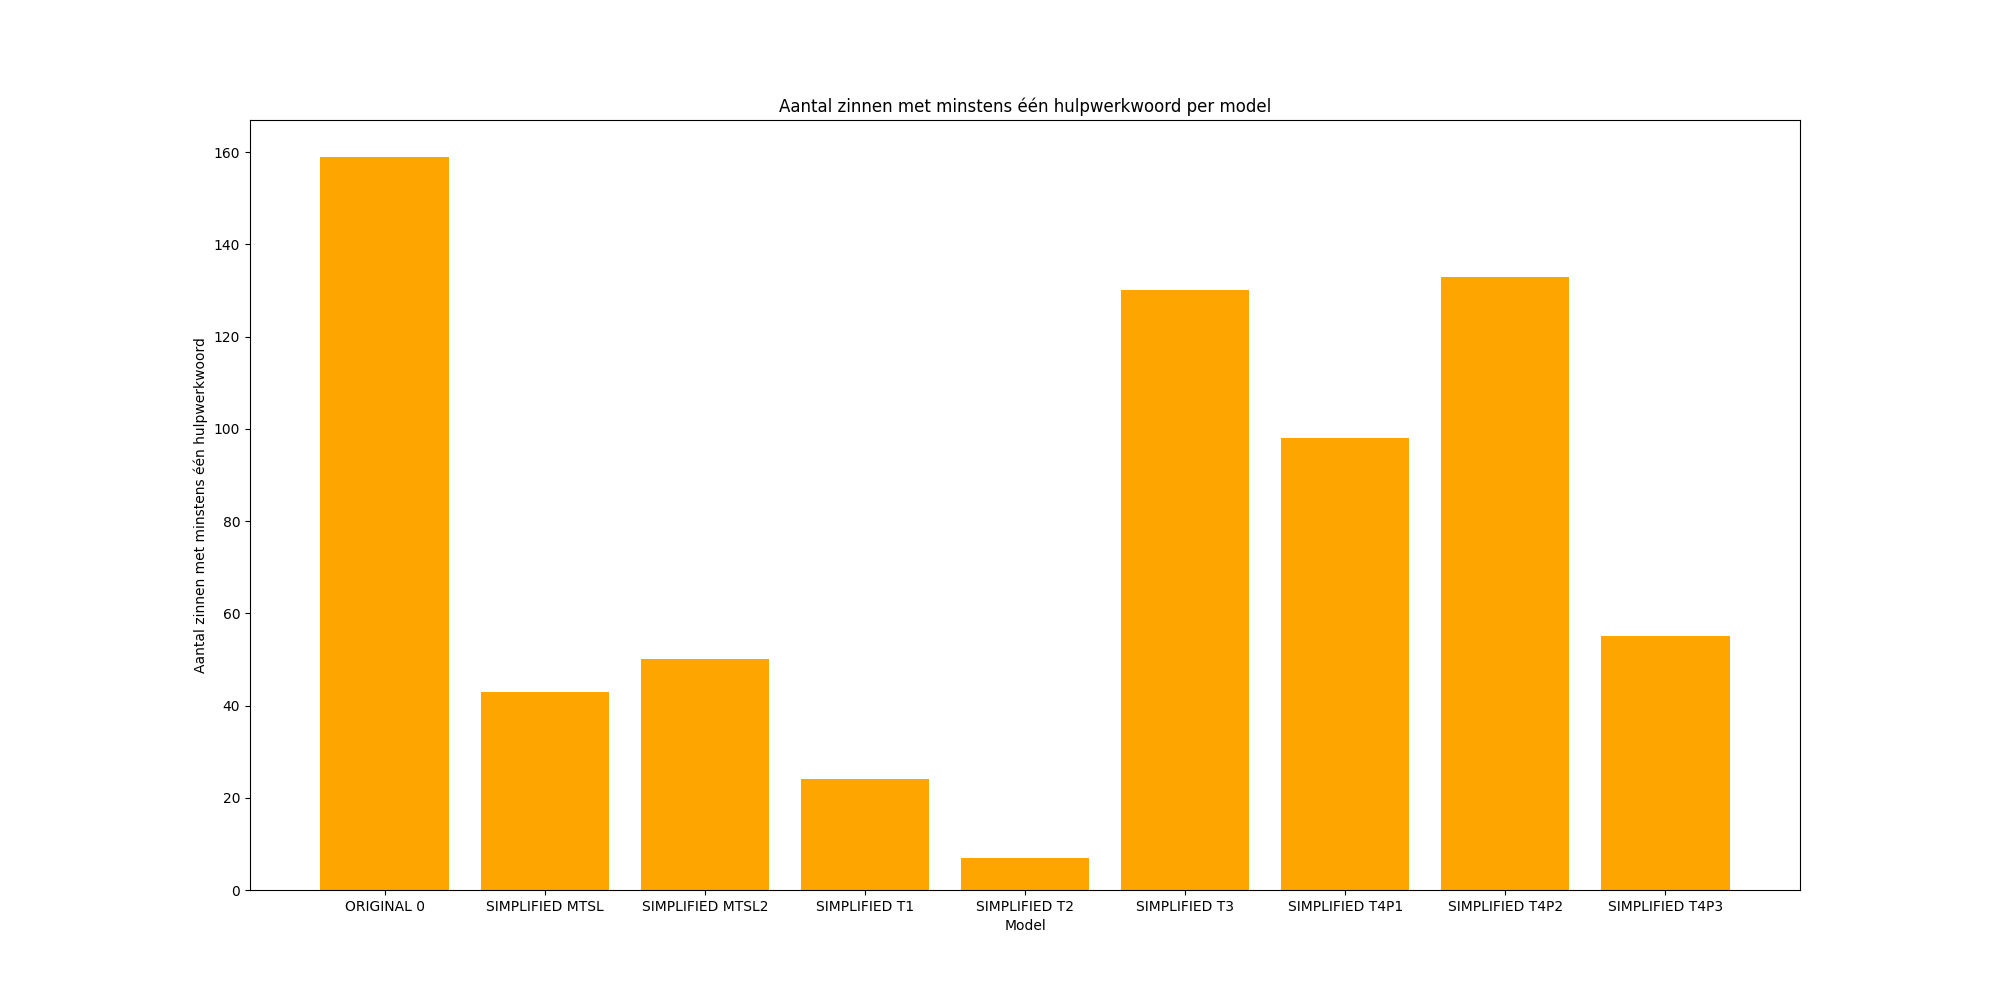
\includegraphics[width=\linewidth]{img/boxplot-aux-a2.png}
	\caption{Een staafdiagram van het aantal gebruikte hulpwerkwoorden in de tekst, gegroepeerd op model voor A2.}
	\label{img:histplot-aux-a2}
\end{figure}

\begin{figure}[H]
	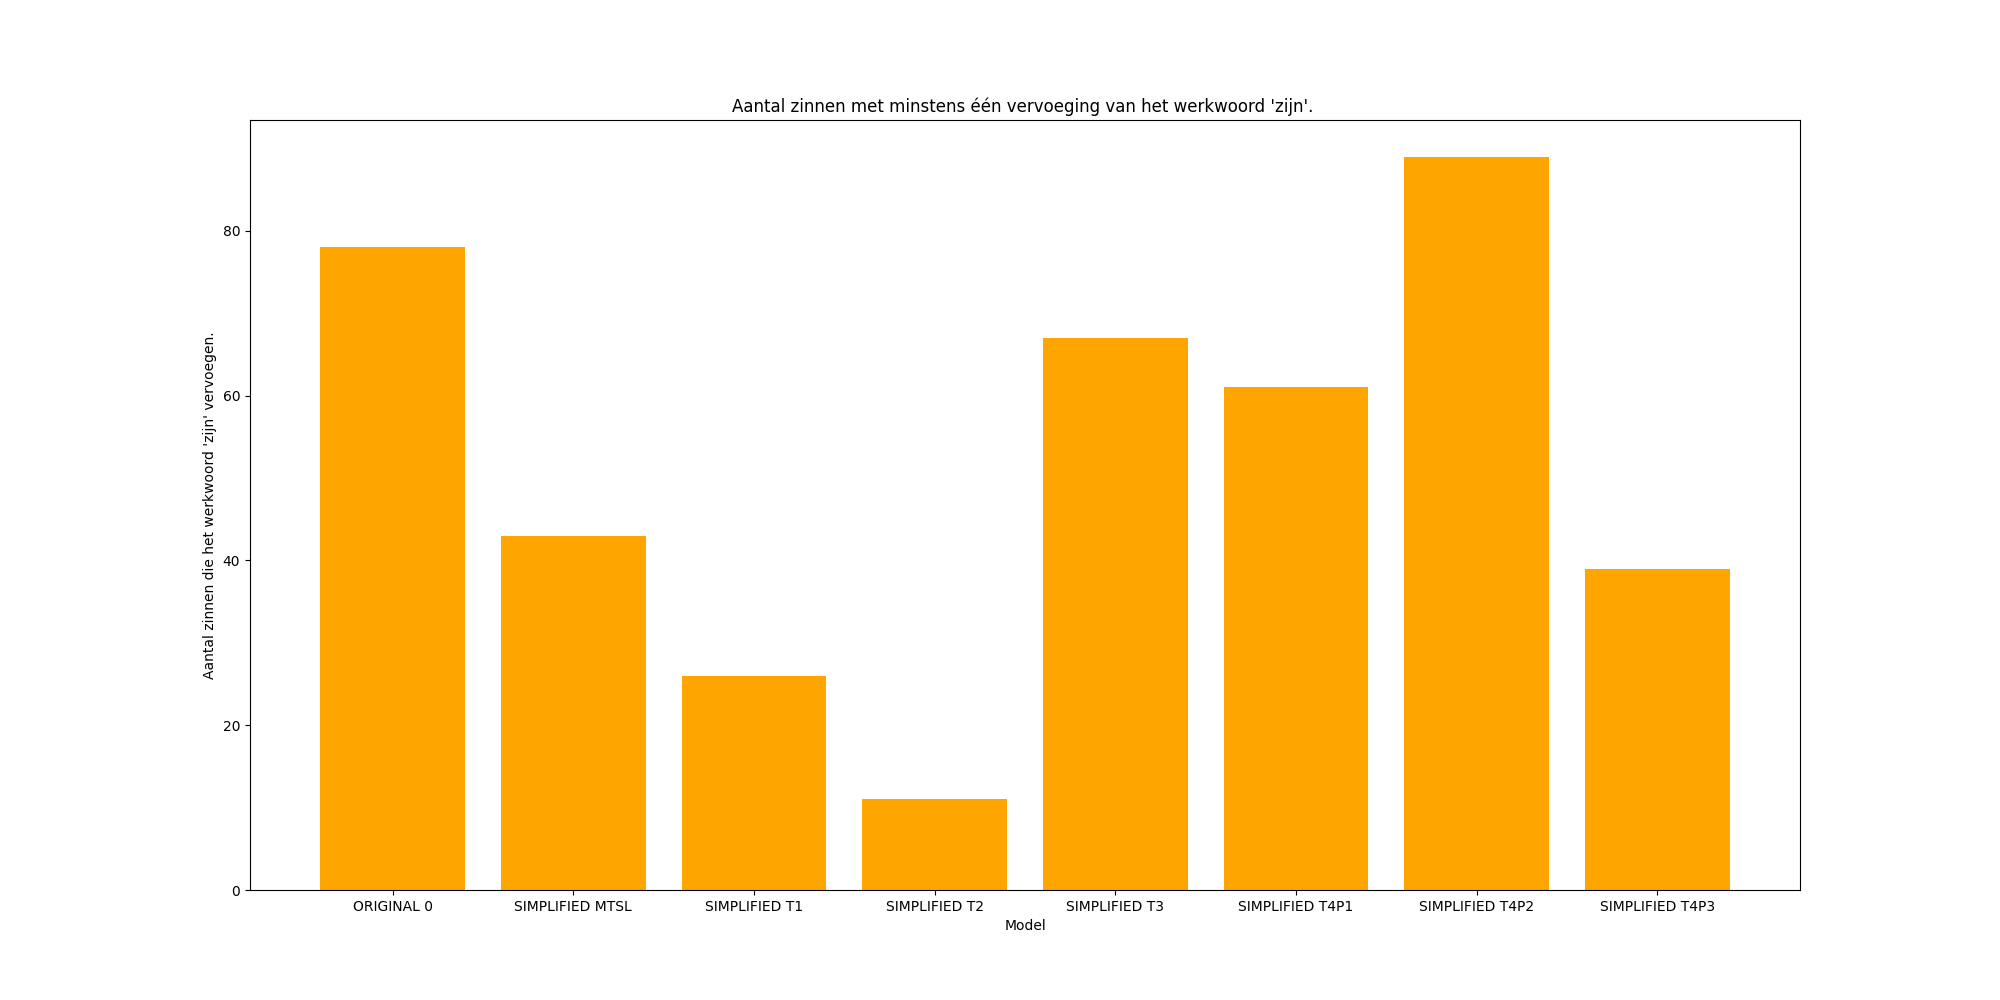
\includegraphics[width=\linewidth]{img/boxplot-tobe-a1.png}
	\caption{Het aantal vervoegingen van het werkwoord 'zijn', gegroepeerd op model voor A1.}
	\label{img:histplot-tobe-a1}
\end{figure}

\begin{figure}[H]
	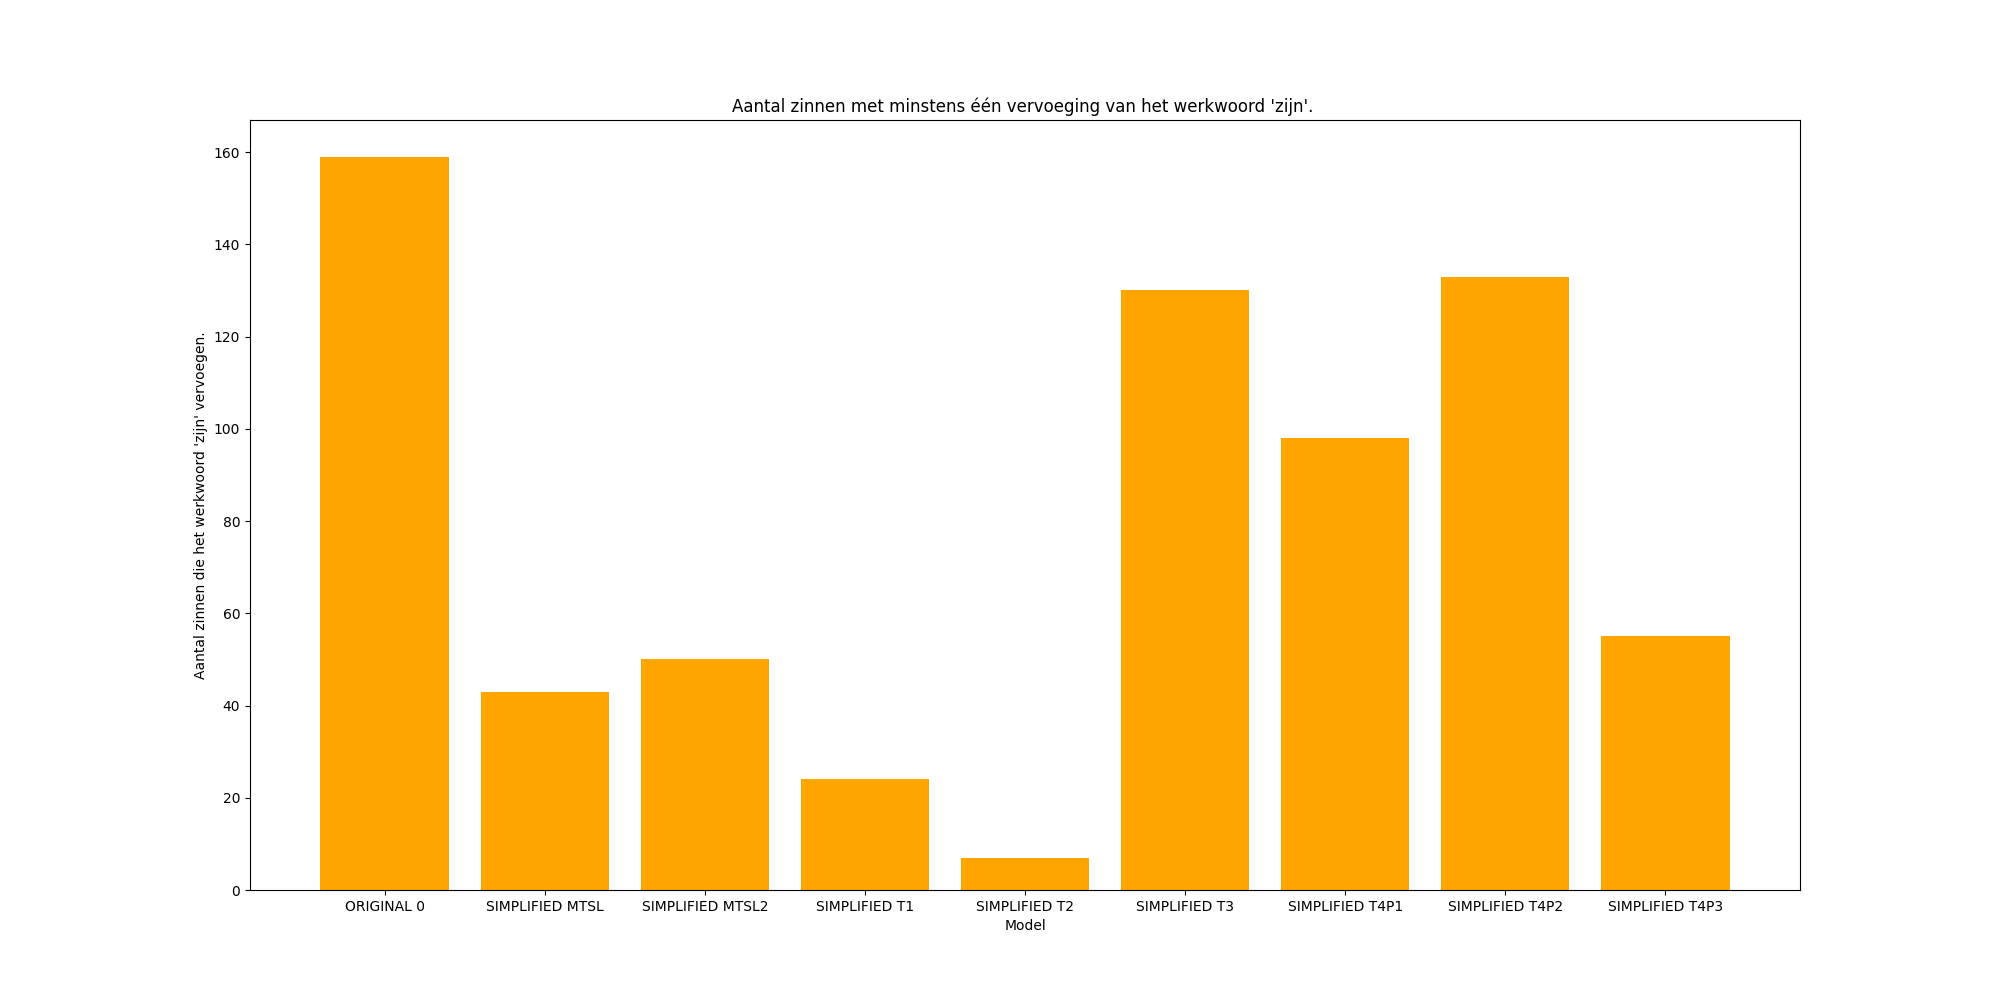
\includegraphics[width=\linewidth]{img/boxplot-tobe-a2.png}
	\caption{Het aantal vervoegingen van het werkwoord 'zijn', gegroepeerd op model voor A2.}
	\label{img:histplot-tobe-a2}
\end{figure}

\subsubsection{Menselijke beoordeling van de referentieteksten.}

In het volgende deel bespreekt het onderzoek de menselijke beoordeling van de resultaten. Allereerst kunnen T4P1 en T4P2 Engelstalige vaktermen vertalen naar het Nederlands. Zo blijft de afkorting voor 'DPKIA' intact, maar vertaalt T4P1 hetzelfde woord naar het Nederlands.  T1, T2, T3 en T4P3 houden hier echter geen rekening mee en behouden de oorspronkelijke versie van de tekst. De auteurs schrijven alle afkortingen voluit, zoals beschreven in de richtlijnen. Zo toont figuur \ref{img:vergelijking-taalmodellen} deze verschillen.

\begin{figure}[H]
	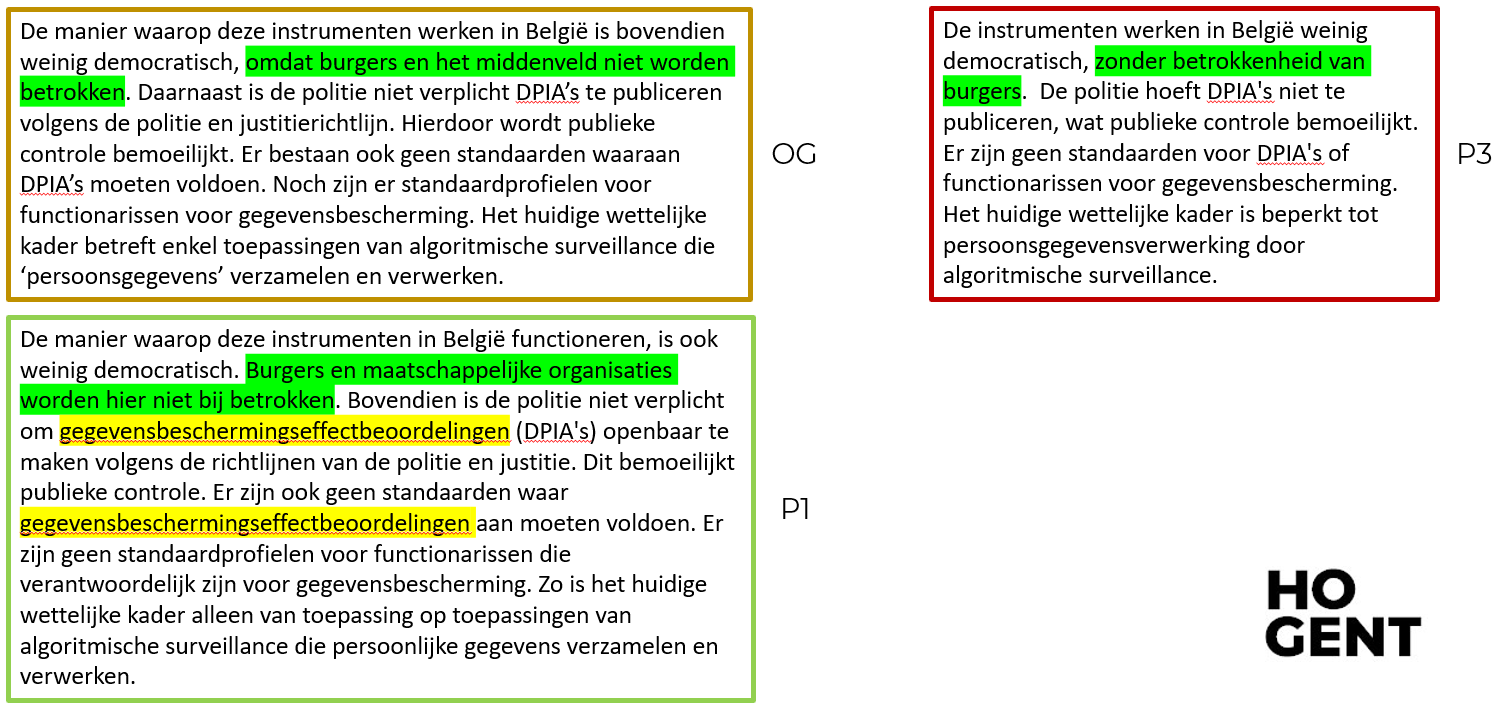
\includegraphics[width=\linewidth]{img/vergelijking.png}
	\caption{De verschillen tussen de oorspronkelijke tekst, T4P1 en T4P3 bij één uitgekozen paragraaf.}
	\label{img:vergelijking-taalmodellen}
\end{figure}

Alle taalmodellen kunnen LS toepassen. De handmatig vereenvoudigde referentieteksten bevatten zinnen die vakjargon gebruiken op het niveau van 15 tot 18 jarige studenten. T4P1 kan uitleg tussen ronde haakjes schrijven, wanneer het geen eenvoudiger synoniem kan vinden. T4P1, T1, T2 en T3 passen woorden aan, maar schrijven geen extra uitleg. T4P3 past deze techniek minder toe dan de vooraf vermelde taalmodellen. T4P3 verkort lange zinnen door deze op te splitsen. T1, T2 en T3 behalen een gelijke zinslengte als dat van de oorspronkelijke zin. T4P1 en T4P2 kunnen langere zinnen genereren, maar smelten geen twee zinnen met elkaar samen. 

\medspace

Geen taalmodel wijkt af van de hoofdgedachte van het oorspronkelijke wetenschappelijk artikel. Hoewel T1, T2 en T3 deels afgebroken zinnen kan genereren, bevatten deze zinnen de hoofdgedachte. T2 bevat minder dan 10\% van het oorspronkelijk artikel en ontbreekt daarbij bijzaken die nodig zijn om alle vragen in \ref{ch:referentietekst} te kunnen begrijpen en te beantwoorden. Tenslotte verwerken T1, T2 en T3 de APA- en California bronvermeldingen niet in de vereenvoudigde teksten. Hoewel T4 deze wel verwerkt, bevat de tekst na een vereenvoudiging deze bronvermeldingen niet meer.

\medspace

Ter conclusie van de resultaten scoren de drie prompts van T4 beter bij de menselijke beoordeling van de resultaten. Het taalmodel en de verwante drie prompts genereren coherente teksten met een verlaagde lexicale complexiteit. Echter houden de geteste taalmodellen weinig tot geen rekening met afkortingen of bronvermeldingen.

\section{Pentimentor vergelijken met \textit{top-of-the-line} tools.}

Gebruikers kunnen vanuit de homepagina drie schermen kiezen: het lerarencomponent, het scholierencomponent en een instellingenpagina. Op de instellingenpagina kunnen eindgebruikers hun persoonlijke opmaak toevoegen. Zo toont figuur \ref{img:website-instellingen} alle mogelijke opmaakopties die Pentimentor aanreikt.

\begin{center}
	\begin{figure}[H]
		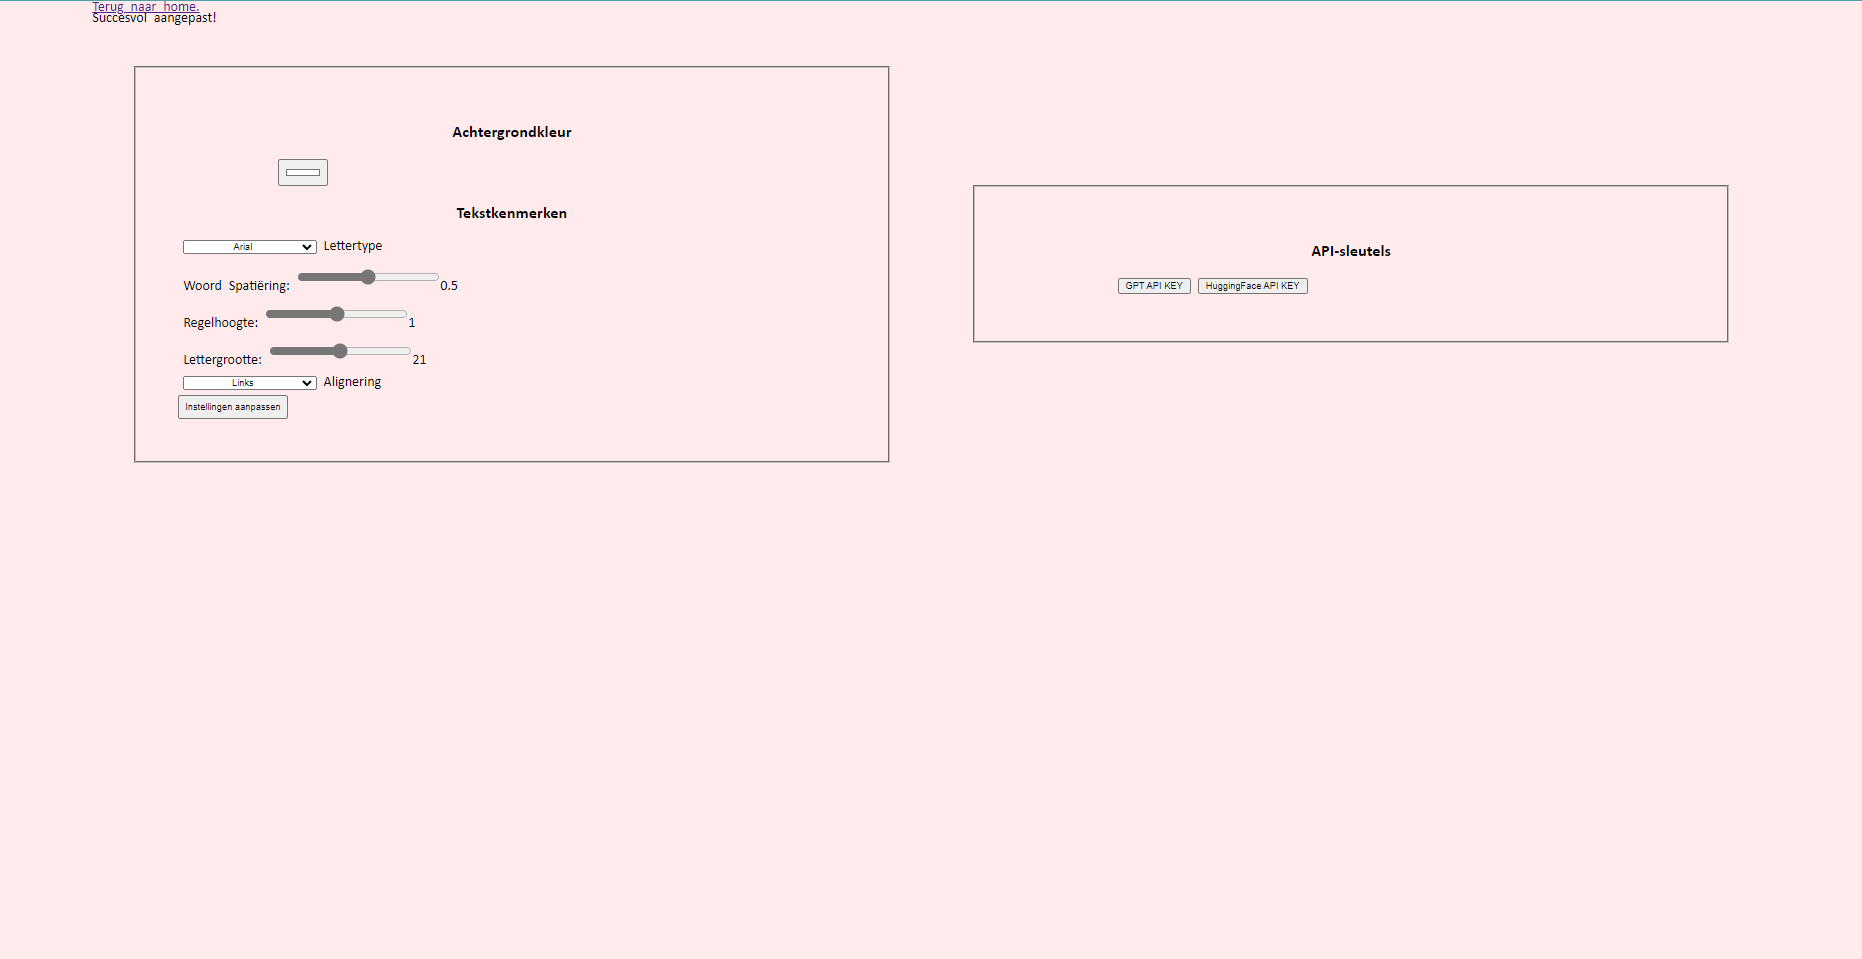
\includegraphics[width=\linewidth]{img/website-instellingen.png}
		\caption{Voorbeeldweergave van de instellingenpagina.}
		\label{img:website-instellingen}
	\end{figure}
\end{center}

Bovendien stelt Pentimentor gebruikers in staat om op basis van gekregen parameters automatisch personaliseerbare docx-documenten te genereren. Zo toont figuur \ref{img:proto-pos-tagging-scholieren} een voorbeeldweergave van deze functionaliteit.

\begin{center}
	\begin{figure}[H]
		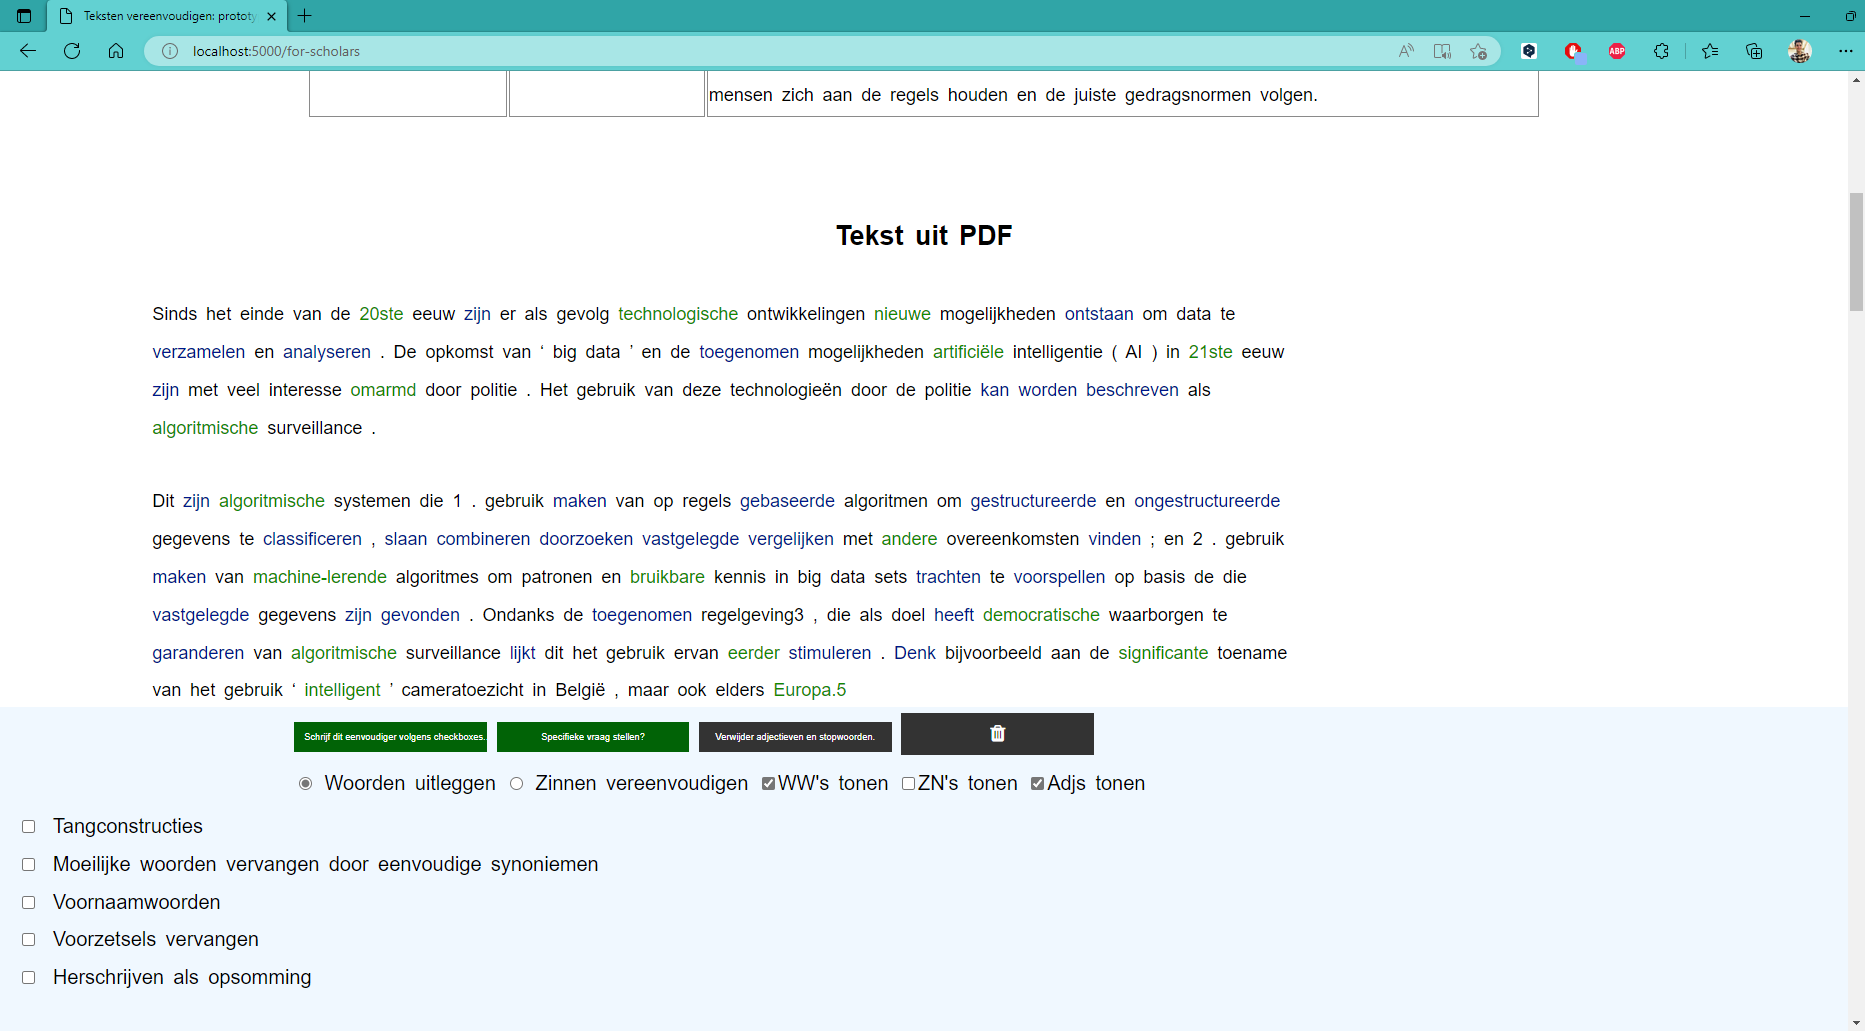
\includegraphics[width=\linewidth]{img/proto-pos-tagging.png}
		\caption{Een voorbeeldweergave van de toepassing van PoS-tagging bij het scholierencomponent.}
		\label{img:proto-pos-tagging-scholieren}
	\end{figure}
\end{center}

Scholieren kunnen zinnen selecteren om daarna deze tekst te laten vereenvoudigen met gepersonaliseerde ATS. Figuren \ref{img:proto-scholieren-step-1} en \ref{img:proto-scholieren-step-3} tonen hoe gebruikers met Pentimentor de gemarkeerde doorlopende tekst kunnen laten herschrijven naar een opsomming. Eerst markeren zij een stuk tekst om hiermee opties aan het mee te geven. Daarnaast kan het ook tekst herschrijven in een tabelformaat.

\begin{center}
	\begin{figure}[H]
		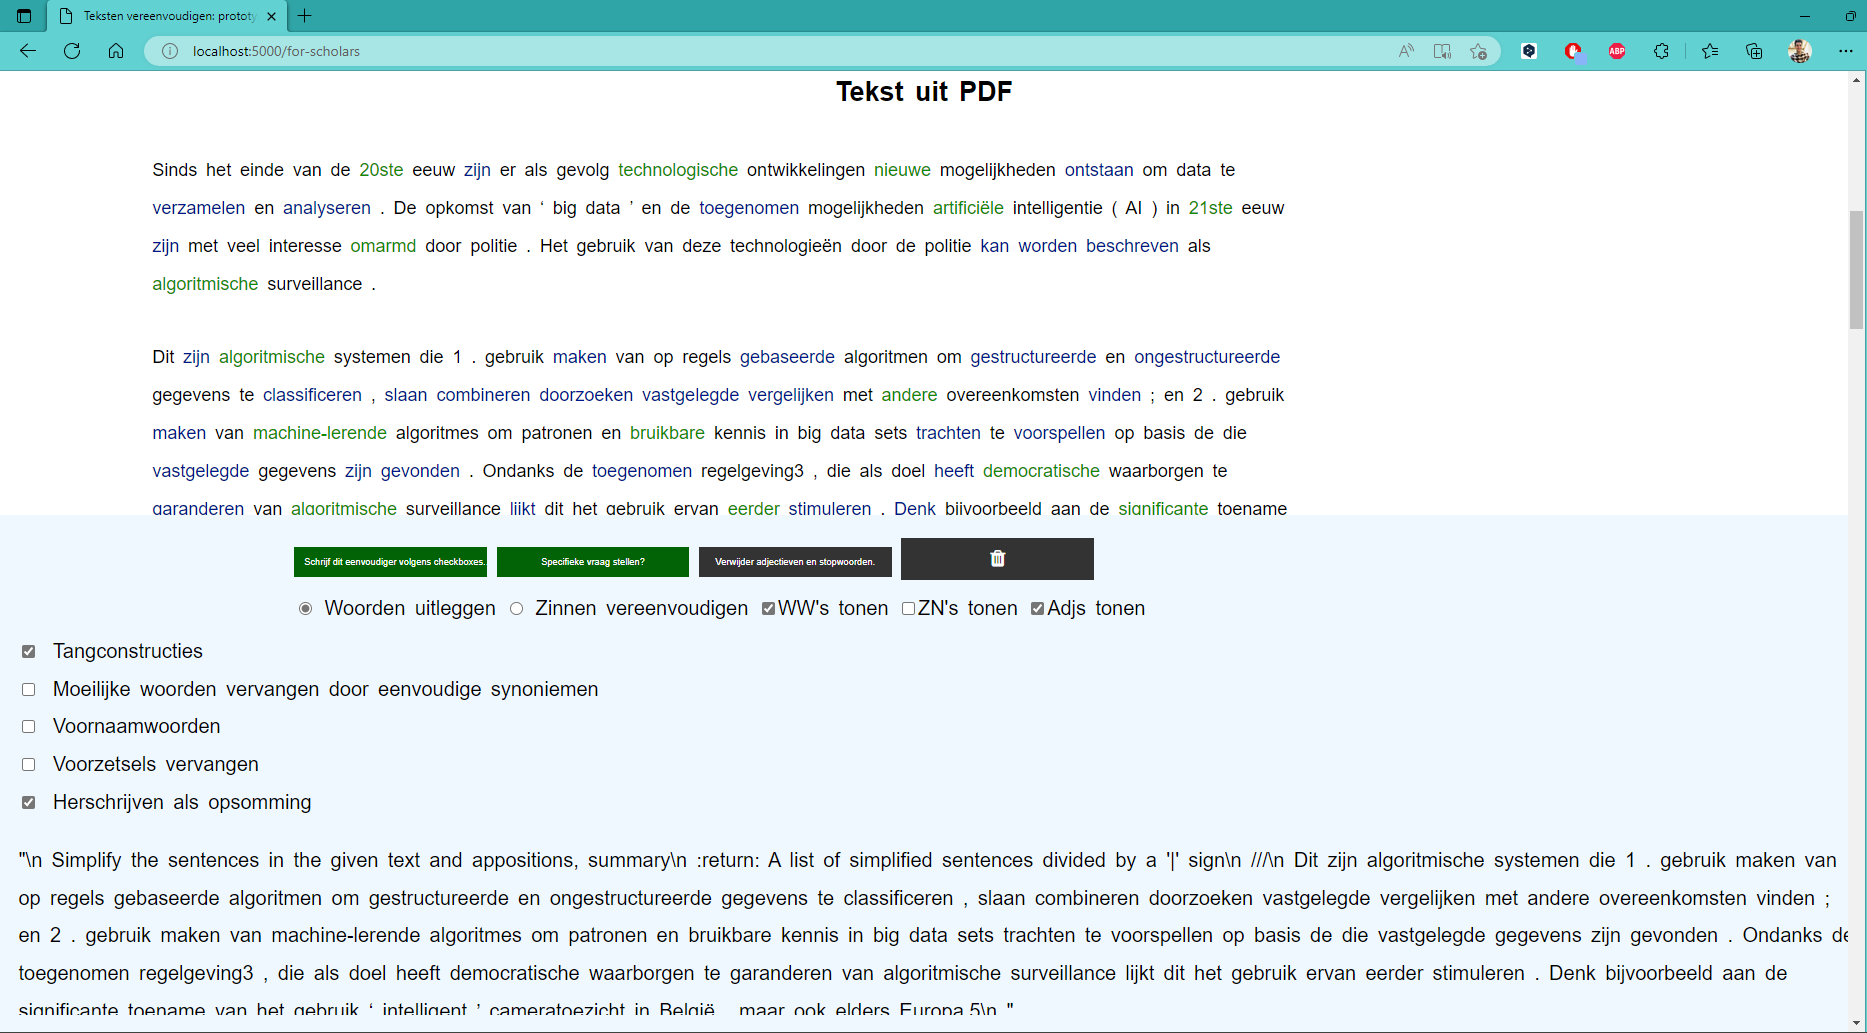
\includegraphics[width=\linewidth]{img/proto-opsomming-1.png}
		\caption{Stap 1 van een gepersonaliseerde tekstvereenvoudiging in het scholierencomponent.}
		\label{img:proto-scholieren-step-1}
	\end{figure}
\end{center}

\begin{center}
	\begin{figure}[H]
		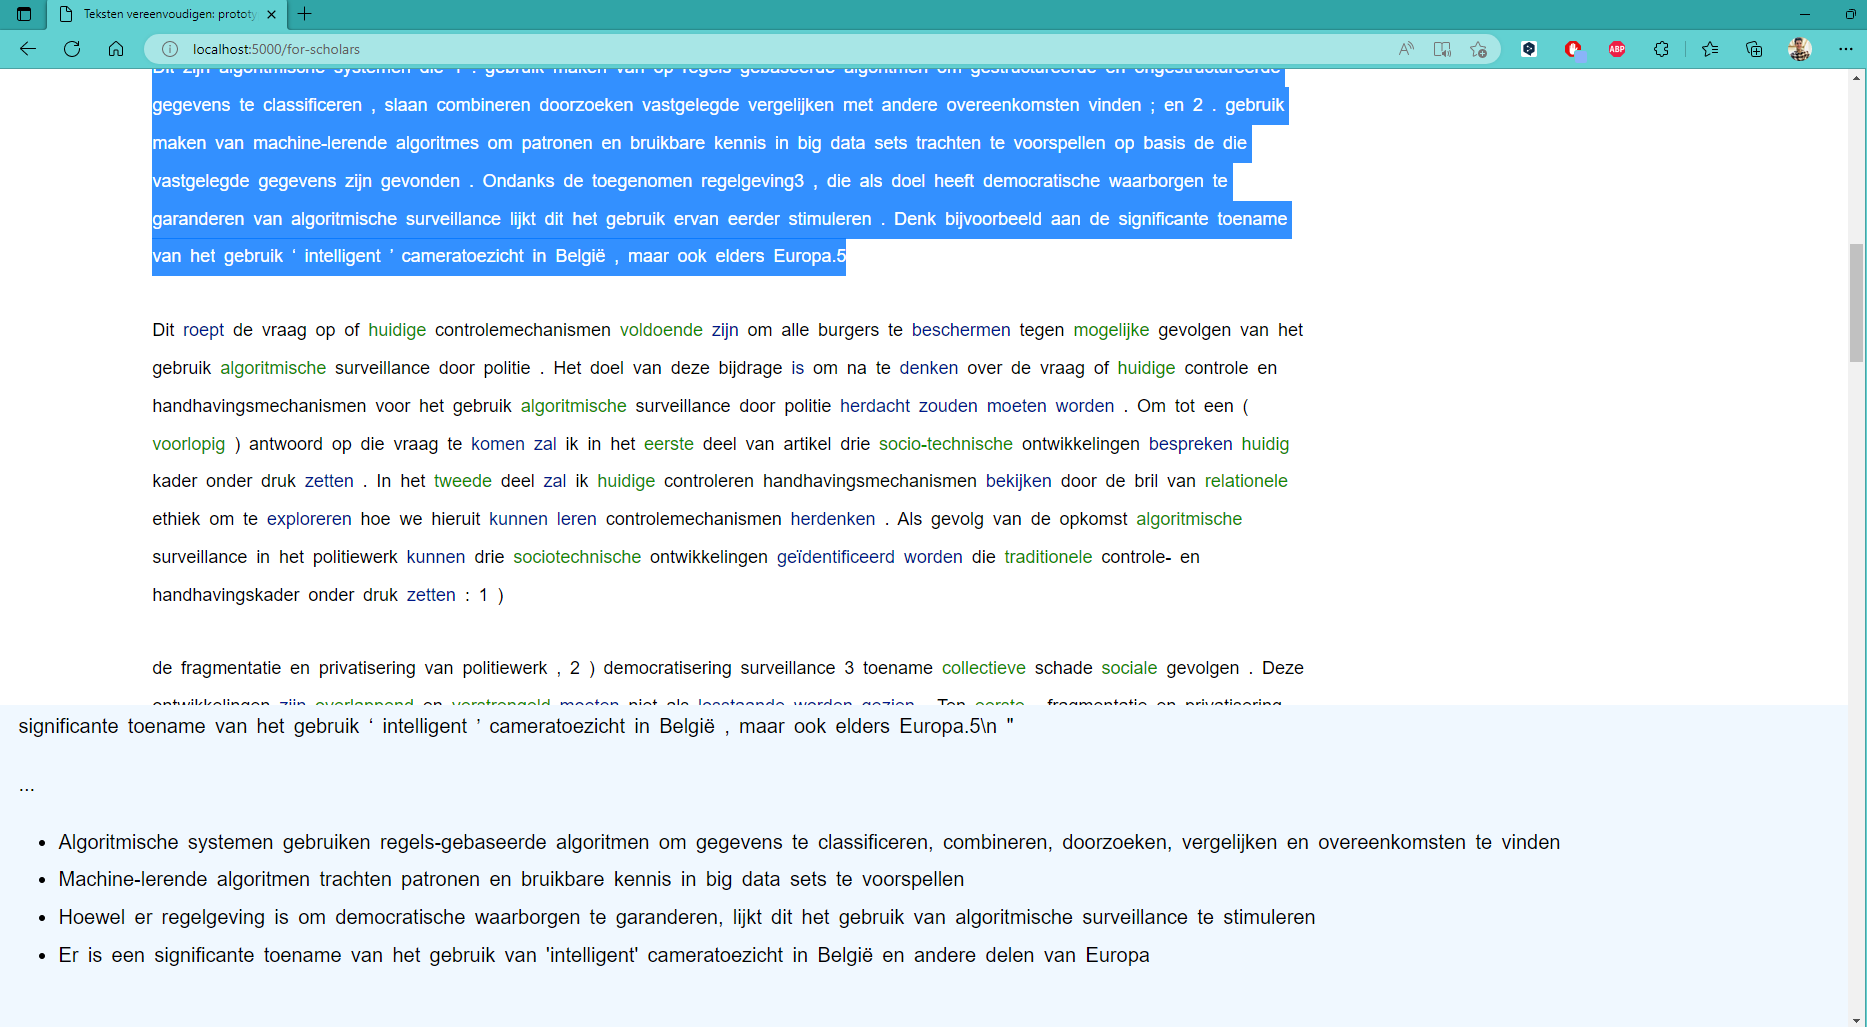
\includegraphics[width=\linewidth]{img/proto-opsomming-3.png}
		\caption{Stap 2 van een gepersonaliseerde tekstvereenvoudiging in het scholierencomponent.}
		\label{img:proto-scholieren-step-3}
	\end{figure}
\end{center}

Verder tonen figuren \ref{img:step-1-proto-vraagstelling} en \ref{img:step-2-proto-vraagstelling} een tweede functionaliteit. Zo kunnen scholieren specifieke vragen stellen aan Pentimentor door middel van een gecentreerd invoerscherm.

\begin{center}
	\begin{figure}[H]
		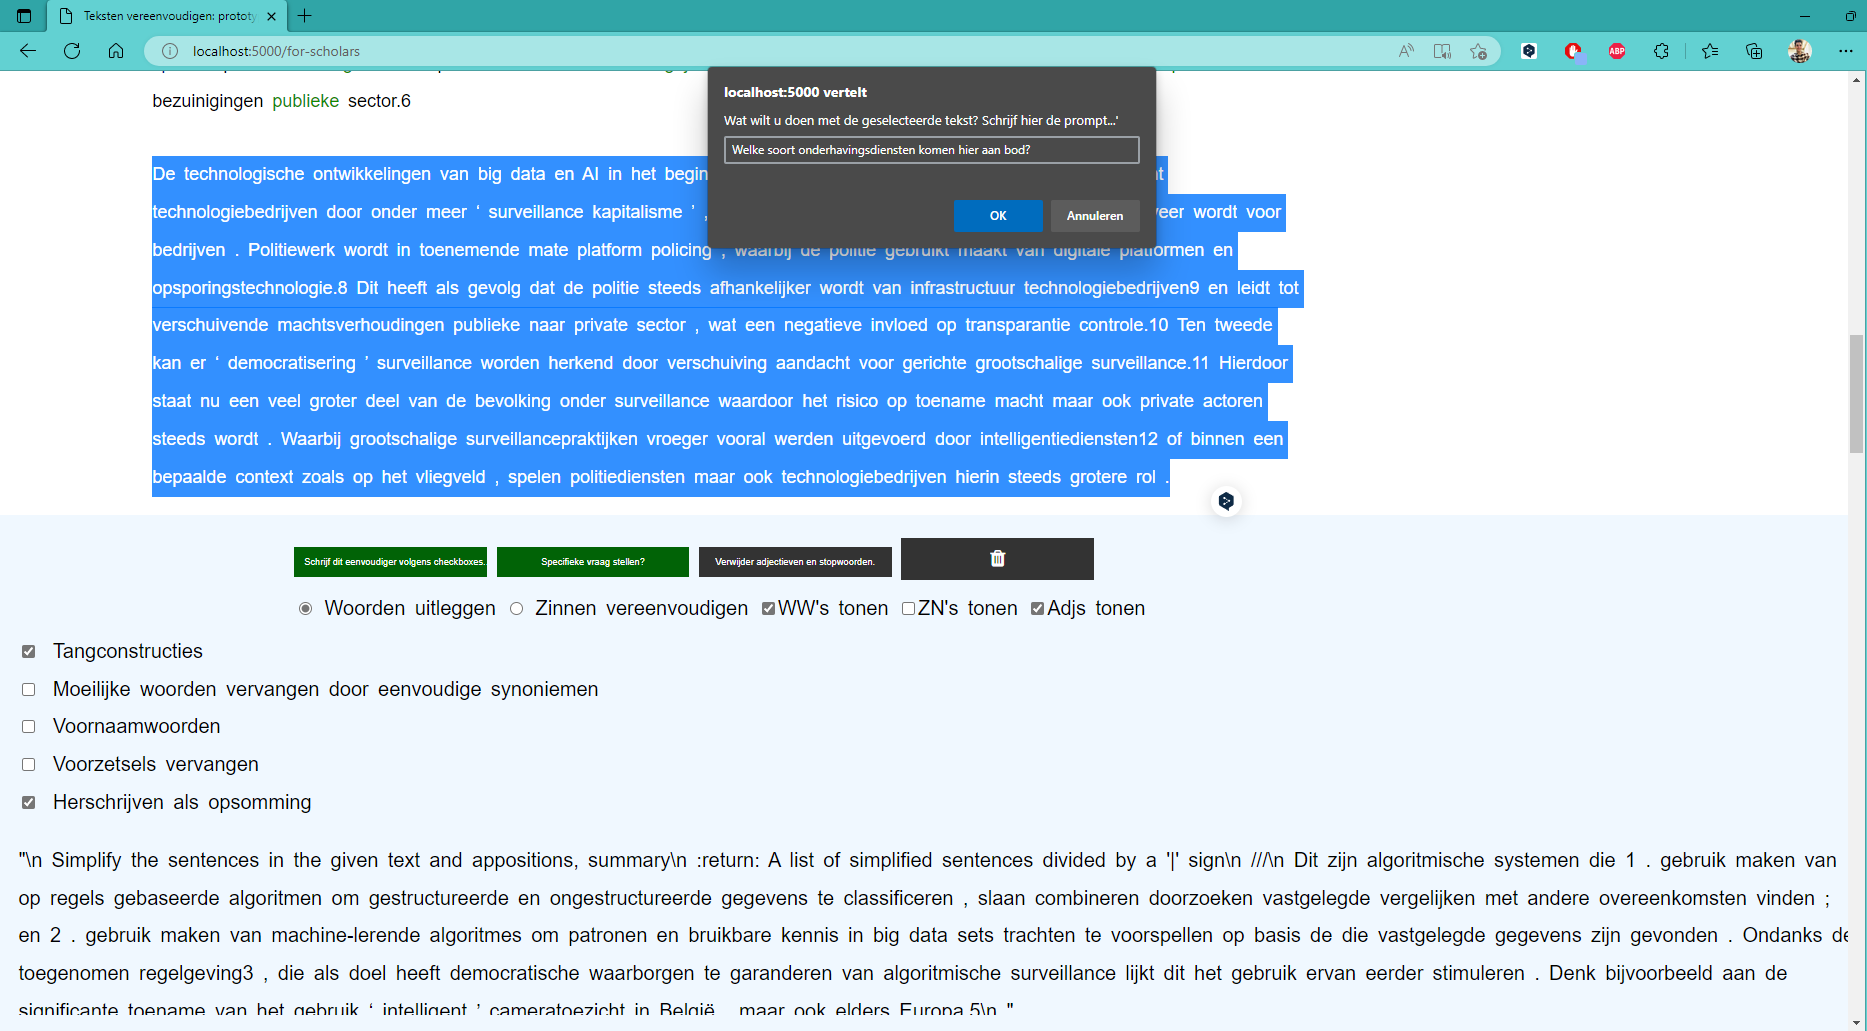
\includegraphics[width=\linewidth]{img/proto-vraagstelling-1.png}
		\caption{Stap 1 bij het stellen van een specifieke vraag bij gemarkeerde tekst.}
		\label{img:step-1-proto-vraagstelling}
	\end{figure}
\end{center}

\begin{center}
	\begin{figure}[H]
		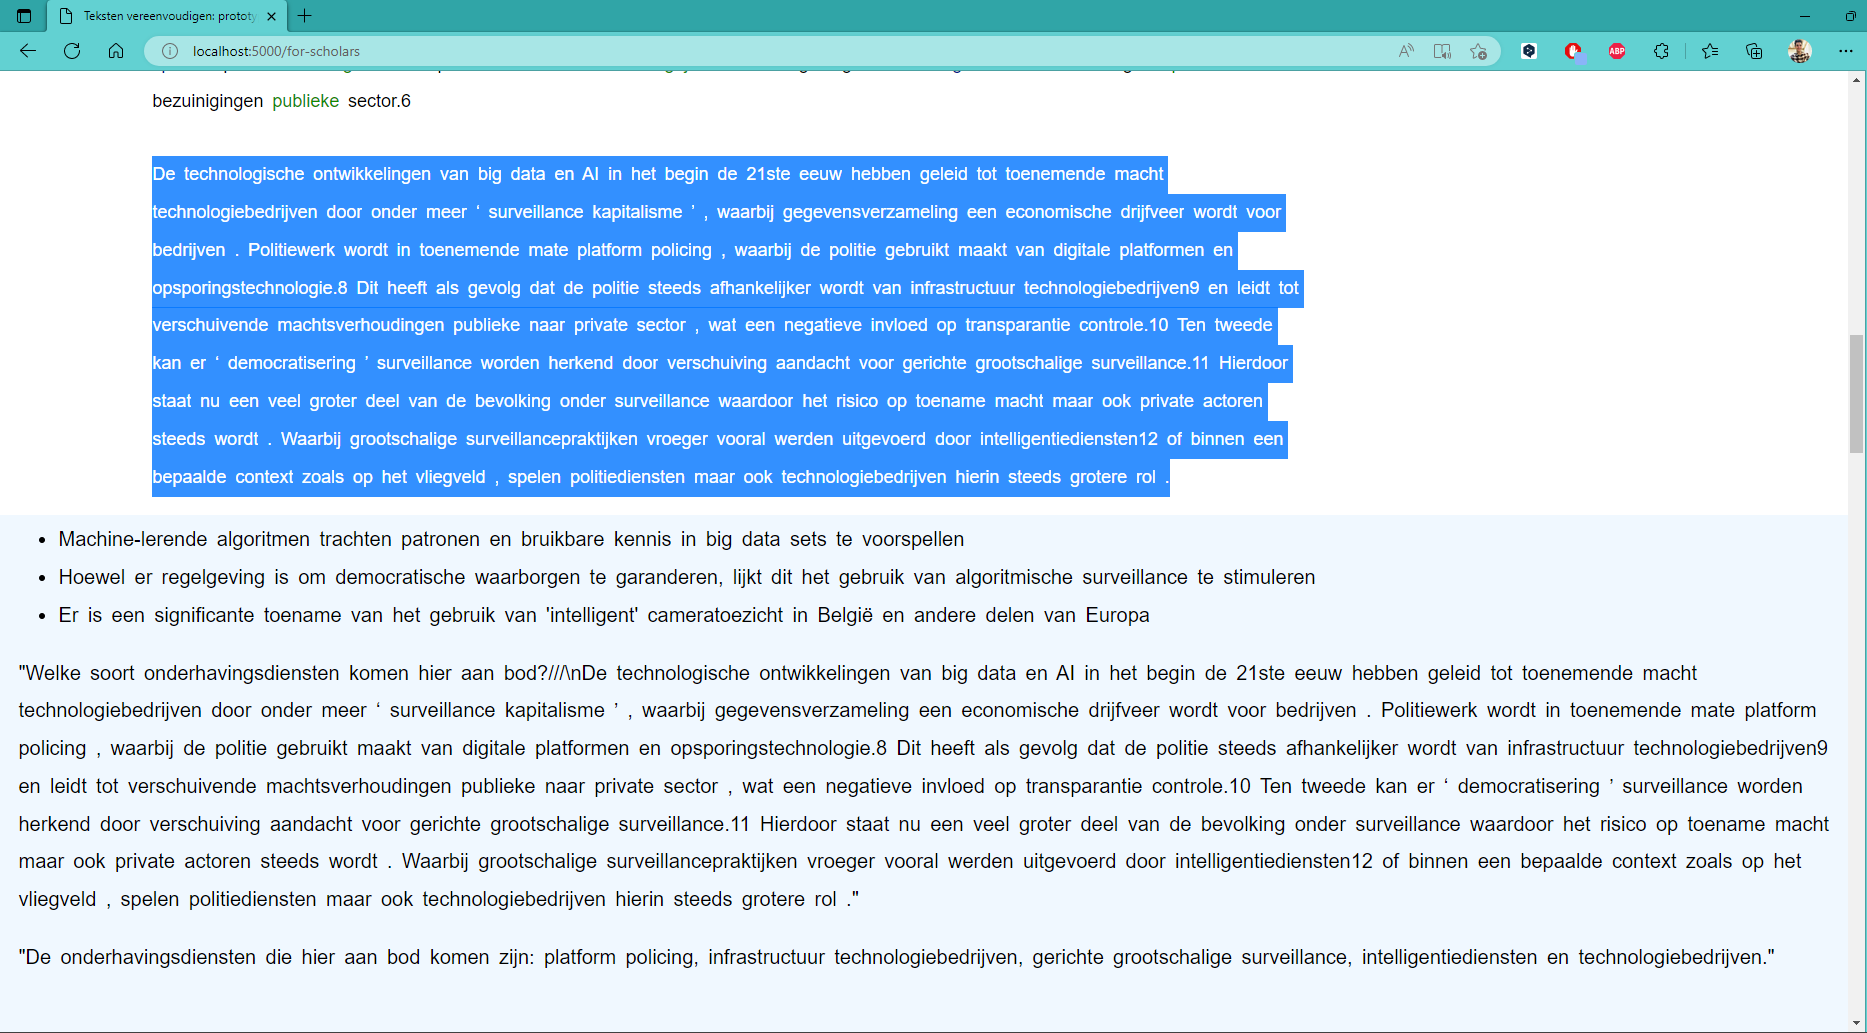
\includegraphics[width=\linewidth]{img/proto-vraagstelling-2.png}
		\caption{Stap 2 bij het stellen van een specifieke vraag bij gemarkeerde tekst.}
		\label{img:step-2-proto-vraagstelling}
	\end{figure}
\end{center}

Volgens de evaluatie en experimenten blijkt Pentimentor te voldoen aan de \textit{must-haves} uit de requirementsanalyse. Tabel \ref{img:moscow-table} geeft hier een overzicht van. Het biedt twee methoden aan om pdf-bestanden in te lezen. Dit via een pipeline van machineleer- en OCR-technieken. Bovendien kan het de tekst ophalen met behulp van PDFMiner, wat overeenkomt met de verwachte functionaliteiten voor pdf-upload. Daarnaast hebben gebruikers de vrijheid om te kiezen welke tekstinhoud ze willen vereenvoudigen met behulp van gepersonaliseerde ATS. Na de vereenvoudiging of samenvatting van een wetenschappelijk artikel kunnen eindgebruikers alle vragen beantwoorden met behulp van de inhoud van het vereenvoudigde artikel, zoals aangegeven door Hollenkamp (2020) als een absolute vereiste.

\medspace

Verder kunnen gebruikers de opmaak van Pentimentor aanpassen naargelang hun voorkeur. Zo past het systeem deze voorkeuren toe op de digitale weergave in de webtool, maar ook de opmaak van het uitvoerbestand. Figuur \ref{img:screenshot-pdf-attempt} toont de vereenvoudigde versie van het wetenschappelijke artikel met de parameters uit tabel \ref{table:chosen-parameters-experiment}. Daarnaast houdt Pentimentor rekening met de gekozen regeleindes, woord- en karakterspatiëring, lettertype -en grootte, koppenstructuur en marges van het uitvoerbestand. Pentimentor houdt hier rekening mee, in tegenstelling tot de andere uitgeteste toools. Enkel E1 en E2 kunnen het lettertype -en grootte aanpassen. Tot slot toont figuur \ref{img:screenshot-docx-attempt} hoe een volledig personaliseerbaar docx-bestand er uit kan zien.

\begin{figure}[H]
	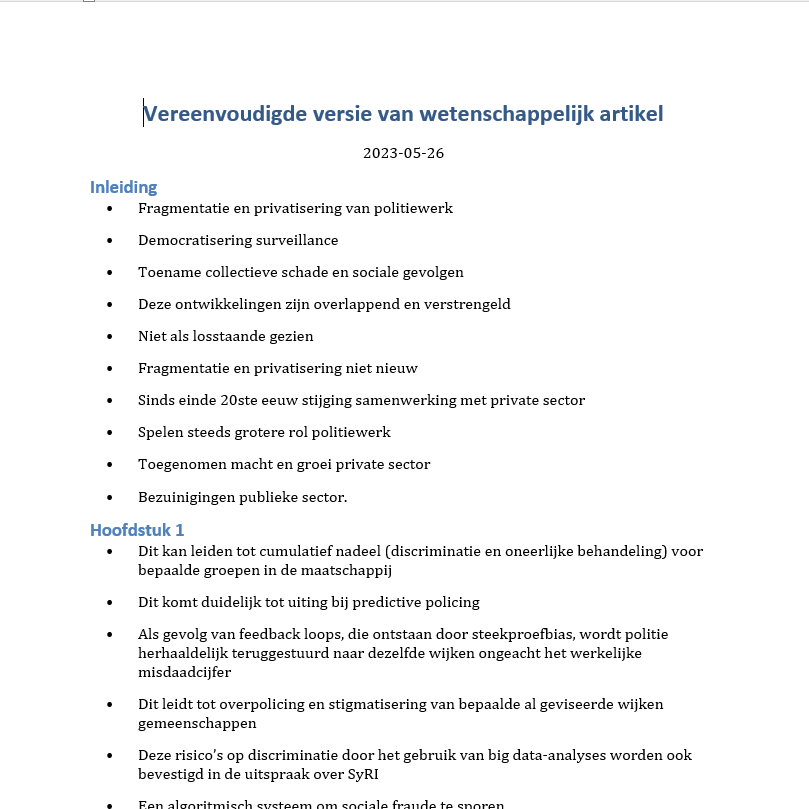
\includegraphics[width=\linewidth]{img/screenshot-prototype-word.png}
	\caption{De uitvoer na een vereenvoudiging met Pentimentor. De tekst is een vereenvoudigde versie van het artikel van \textcite{VanBrakel2022}.}
	\label{img:screenshot-docx-attempt}
\end{figure}

Verder bevat Pentimentor enkele \textit{should-haves}. Allereerst kunnen gebruikers een tekst op een duidelijke manier markeren. Hiermee kunnen zij annotaties toevoegen, de tekst aanpassen door \textit{in-line} definities toe te voegen. Bovendien kan Pentimentor abstraherende samenvattingen genereren in verschillende formaten, zoals opsommingen, tabellen of doorlopende tekst. Zo toont figuur \ref{img:screenshot-docx-attempt} een voorbeeld van een gegenereerde opsommingssamenvatting.

\medspace

Pentimentor zorgt voor een duidelijke gebruikerservaring door meldingsschermen te tonen wanneer het iets van de gebruiker verwacht. Figuur \ref{img:step-1-proto-vraagstelling} illustreert deze werking. Bovendien toont het waarschuwingen in formulieren, zoals getoond in figuur \ref{img:proto-lerarencomponent}.

\begin{figure}[H]
    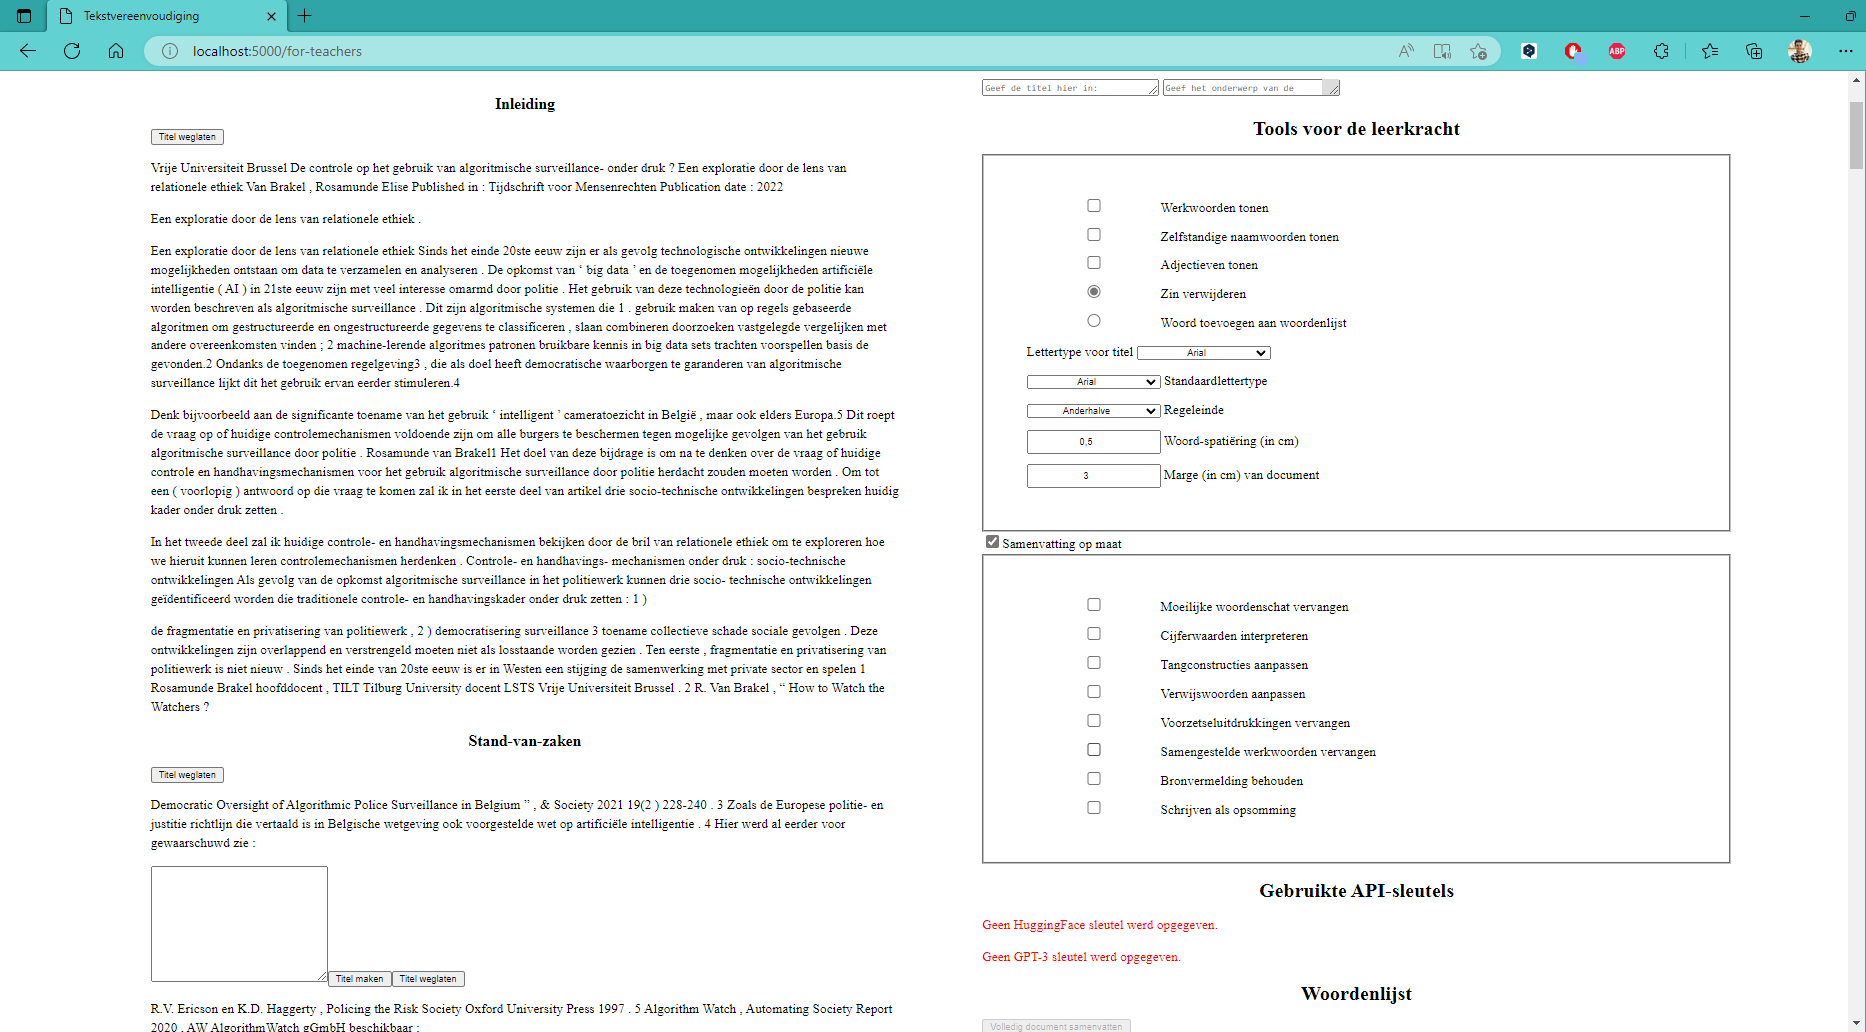
\includegraphics[width=\linewidth]{img/proto-lerarencomponent.png}
    \caption{Een mogelijke weergave van het lerarencomponent met het wetenschappelijk artikel van \textcite{VanBrakel2022} als input.}
    \label{img:proto-lerarencomponent}
\end{figure}

Echter voldoet Pentimentor niet aan alle \textit{should-haves}. Zo ontbreekt de mogelijkheid om automatisch een woordenlijst met moeilijke woorden of vakjargon te genereren. Daarnaast mist Pentimentor analytische functionaliteiten, zoals het tonen van tekstanalyse aan de eindgebruiker.

\medspace

Tot slot bevat Pentimentor geen \textit{wont-haves}. Zo ontbreekt het een luistercomponent waarmee scholieren de vereenvoudigde tekst kunnen beluisteren. Deze functionaliteit is wel aanwezig bij E1, E2 en E3. Andere uitgeteste tools beschikken hier ook niet over. Bovendien kunnen gebruikers Pentimentor alleen raadplegen in een lokale omgeving met Docker, terwijl zij wel andere geteste toepassingen zonder installatie kunnen raadplegen. Daarnaast heeft Pentimentor geen browserextensie, terwijl O5 dit als enige toepassing wel kan.